\documentclass[11pt,a4paper]{article}

% ---------- Packages ----------
\usepackage[margin=1in]{geometry}
\usepackage{amsmath, amssymb, amsthm, mathtools}
\usepackage{microtype}
\usepackage{graphicx}
\usepackage{booktabs}
\usepackage{enumitem}
\usepackage{xcolor}
\usepackage[colorlinks=true,
            linkcolor=blue!50!black,
            urlcolor=blue!50!black,
            citecolor=blue!50!black]{hyperref}

% Figures are generated by experiments/make_figures.py.
\graphicspath{{../results/figures/}}

% ---------- Theorem environments ----------
\theoremstyle{plain}
\newtheorem{theorem}{Theorem}[section]
\newtheorem{proposition}[theorem]{Proposition}
\newtheorem{lemma}[theorem]{Lemma}
\newtheorem{corollary}[theorem]{Corollary}

\theoremstyle{definition}
\newtheorem{definition}[theorem]{Definition}

\theoremstyle{remark}
\newtheorem{remark}[theorem]{Remark}

% ---------- Notation (as in the thesis) ----------
\newcommand{\R}{\mathbb{R}}
\newcommand{\E}{\mathbb{E}}
\newcommand{\PP}{\mathbb{P}}
\newcommand{\Q}{\mathbb{Q}}
\newcommand{\F}{\mathcal{F}}
\newcommand{\1}{\mathbf{1}}
\newcommand{\dd}{\mathrm{d}}
\newcommand{\eqdef}{\coloneqq}
\newcommand{\Var}{\operatorname{Var}}
\newcommand{\VRF}{\mathrm{VRF}}
\newcommand{\Wt}{\widetilde{W}}
\newcommand{\Qt}{\Q^{\theta}}
\newcommand{\Cov}{\operatorname{Cov}}
\newcommand{\Corr}{\operatorname{Corr}}
\newcommand{\Eff}{\mathrm{Eff}}

% ---------- Document metadata ----------
\title{Importance Sampling via Girsanov's Theorem:\\
       Variance Reduction for Out-of-the-Money Options\\
       under Black--Scholes}
\author{Roberto Cepeda Rocandio}
\date{November 2026}

\begin{document}
\maketitle

\begin{abstract}
Out of the money, plain Monte Carlo loses its relative precision, since almost every simulated path ends out of the money and carries no information about the price. It is natural to ask, then, whether we can sample where the payoff lives and still estimate the same price. This note answers it with the change of measure of Girsanov's theorem, used not to price but to sample: adding a constant drift to the Brownian motion under which we simulate, and weighting each sample by the likelihood ratio, gives an unbiased estimator whose variance is a weighted second moment. For the European call and the cash-or-nothing digital under Black--Scholes this second moment has a closed form, and it is strictly convex in the drift and grows without bound in both directions, so the optimal drift exists and is unique, and it can be compared with a simple heuristic that centres the terminal price at the strike. The experiments confirm what the theory predicts: out of the money the variance falls by orders of magnitude, far more than the extra cost of the weights, near the money the heuristic does worse than plain Monte Carlo, and antithetic variates give nothing precisely where importance sampling gains most. We close with the limits of the method, the confidence interval without hits and the degenerate weights of an excessive drift, which turn out to be one and the same failure, and with a short pilot run that finds the optimal drift without its closed form. The method is classical, and the aim of the note is a detailed account of it, built on the bachelor's thesis that it continues, in the simplest setting where every quantity can be checked against a closed form. A single script reproduces the figures and the table.
\end{abstract}

\section{Introduction}
\label{sec:intro}

The error of a Monte Carlo estimate is governed by the variance of the sampled variable: its standard error, and with it the half-width of the confidence interval, scales like $\sigma_Y/\sqrt n$, so with $n$ fixed the only way to make the estimate more precise is to reduce the variance. This is the starting point of variance reduction, and it raises the question this note is about: is it worth paying some extra computation per sample to estimate the same price through a different random variable, with the same expectation and a smaller variance, and so obtain narrower confidence intervals? The question is not academic. Out of the money almost no simulated path ends in the money, so almost every sample of the discounted payoff is zero, and plain Monte Carlo loses its relative precision: the problem is not that the price is small, but that almost every sample carries no information about it.

The tool we use comes from the bachelor's thesis that this note continues \cite{tfg}. There, the risk-neutral measure is reached through Girsanov's theorem \cite[Thm~4.20]{tfg}, and both its introduction \cite[\S 1.1]{tfg} and the remark that follows the Radon--Nikodym theorem \cite[Remark~4.16]{tfg} point out that replacing a measure by an equivalent one is a device of general use, whose application in simulation is precisely importance sampling. This note develops that remark. We use the same theorem the other way round: instead of removing a drift to reach $\Q$, we add one to the Brownian motion under which we simulate, so that more paths end in the money, and we correct every sample by the likelihood ratio. The drift is then no longer fixed by the absence of arbitrage, as in the thesis, but chosen to reduce the variance, and the two roles never mix: $\Q$ is the measure we price under, and $\Qt$ the one we sample under.

The note also fills a gap. The note on variance reduction of \cite{portfolio}, which covers antithetic and control variates, leaves importance sampling out of its scope \cite[\S 6]{portfolio}, precisely because it does not target the regime in which importance sampling pays, deep out of the money. Here we treat that regime, and we measure importance sampling against antithetic variates, the reference that the portfolio already has, on the same example and with the same convention for comparing estimators.

We should be clear about what this note is and what it is not. None of its ingredients is new: importance sampling by a change of drift is a classical technique \cite[\S 4.6]{glasserman}, and so are the closed-form prices against which we test it. What the note offers is a detailed account of the method, explained step by step, in the simplest setting in which it can be studied completely, the European call and the cash-or-nothing digital under Black--Scholes, an account in which every result about the estimators is proved in the note and the stochastic calculus, from Girsanov's theorem to the Black--Scholes formulas, is taken from the thesis and cited by number. With a constant drift and a payoff that depends only on $S_T$, the change of measure reduces to moving the mean of a single Gaussian variable, the normalised endpoint of the Brownian motion, so every expectation of the note is a one-dimensional Gaussian integral. This is why every quantity of interest has a closed form, from the price to the variance of each estimator, and it is precisely what turns every experiment into a check of the theory against an exact value. What Girsanov's theorem adds to this picture, and what carries over to payoffs that depend on the path (Subsection~\ref{subsec:outlook}), is that the shift is a change of measure on the whole path space.

The note is organised as follows. Section~\ref{sec:mc} sets up plain Monte Carlo under the risk-neutral measure, introduces the call and the digital as benchmarks, fixes how two estimators are compared, by their variance at equal work and by their efficiency, and presents antithetic variates, which will be our reference. Section~\ref{sec:is} is the core of the note: it builds the sampling measure from Girsanov's theorem, writes the likelihood ratio as a function of the simulated normal, proves that the estimator is unbiased and expresses its variance as a weighted second moment. Section~\ref{sec:theta} asks how the drift should be chosen, computes the second moment in closed form, and compares a simple heuristic with the optimal drift, whose existence and uniqueness follow from the shape of the second moment, strictly convex and unbounded in both directions, and which can be read as the Gaussian law nearest to the zero-variance one. Section~\ref{sec:results} puts these predictions next to the measurements, and Section~\ref{sec:limits} gathers the limits of the method, puts to the test the pilot run that estimates the optimal drift without its closed form, and points to the directions in which the method extends. Appendix~\ref{app:table} collects the summary table. The code that produces every figure and the table, together with the tests that check the results of Sections~\ref{sec:mc} to~\ref{sec:theta}, is in the same repository as this note.

\section{Monte Carlo under the risk-neutral measure}
\label{sec:mc}

By \cite[Thm~5.7]{tfg} with $t = 0$, the price of a European derivative with payoff $h(S_T)$ is the expectation $V = \E_\Q[e^{-rT}h(S_T)]$ of \cite[(5.23)]{tfg}, which the thesis computes only when it can be done by hand, as for the call \cite[Thm~5.8]{tfg}. What we need here is something else: to turn the expectation into a number by simulation, to say how far that number may be from $V$, and, since the rest of the note is about replacing one estimator by another, to fix beforehand what it means for one estimator to be better than another. The section closes with antithetic variates, the variance reduction technique of \cite{portfolio} against which importance sampling will be measured.

\subsection{The estimator and its error}

Write $Z \eqdef \Wt_T/\sqrt T$, where $\Wt$ is the $\Q$-Brownian motion of \cite[(5.13)]{tfg}, so that $Z$ is $\mathcal N(0,1)$ under $\Q$. By \cite[(5.26)]{tfg}, $S_T = S_0 \exp\bigl((r - \tfrac12\sigma^2)T + \sigma\sqrt T Z\bigr)$, and the discounted payoff is therefore a function of a single standard normal,
\begin{equation}\label{eq:g}
  Y \eqdef e^{-rT}h(S_T) = g(Z),
  \qquad
  g(z) \eqdef e^{-rT}h\bigl(S_0\, e^{(r - \frac12\sigma^2)T + \sigma\sqrt T z}\bigr),
\end{equation}
with $V = \E_\Q[g(Z)]$. To estimate it, it suffices to draw independent copies of $Z$ and average.

\begin{definition}\label{def:mc}
Let $Z_1, \dots, Z_n$ be i.i.d.\ $\mathcal N(0,1)$ random variables, in practice the draws of a random number generator, and let $Y_i \eqdef g(Z_i)$. The plain Monte Carlo estimator of $V$ is
\begin{equation}\label{eq:mc}
  \hat V_n \eqdef \frac1n \sum_{i=1}^n Y_i .
\end{equation}
\end{definition}

The $Y_i$ are i.i.d.\ copies of $Y$, being the same function of i.i.d.\ inputs, so linearity gives $\E[\hat V_n] = V$ and the strong law of large numbers gives $\hat V_n \to V$ almost surely, $Y$ being integrable, and in fact square integrable, for both payoffs of this note (the digital is bounded by one, and the call by $S_T$, which has moments of all orders \cite[\S 5.3]{tfg}). Now, this says that the estimate is right on average and in the limit, and nothing about how far from $V$ it is for the $n$ we can afford, which is the job of the second moment. Since independence kills the cross terms, $\Var(\hat V_n) = \sigma_Y^2/n$, with $\sigma_Y^2 \eqdef \Var_\Q(Y)$, and the standard error
\begin{equation}\label{eq:se}
  \mathrm{SE}_n \eqdef \frac{\sigma_Y}{\sqrt n}
\end{equation}
is the typical size of the error $\hat V_n - V$. Two things follow from \eqref{eq:se}, and the whole note rests on the second. The first is that Monte Carlo is slow: dividing the error by ten costs a hundred times more samples. The second is that, with $n$ fixed, the only way to reduce the error is to reduce $\sigma_Y$, that is, to replace $Y$ by another random variable with the same expectation and a smaller variance. Antithetic variates (Subsection~\ref{subsec:av}) do it without changing the measure, and importance sampling (Section~\ref{sec:is}) does it by changing it.

To report an interval we also need the shape of the error, and this is what the central limit theorem gives: $\sqrt n\,(\hat V_n - V)/\sigma_Y$ converges in law to $\mathcal N(0,1)$, whatever the law of $Y$, which here is far from Gaussian (a scaled Bernoulli variable for the digital, a point mass at zero plus a lognormal tail for the call). The unknown $\sigma_Y$ is replaced by the sample standard deviation $s_n$, with $s_n^2 \eqdef \frac{1}{n-1}\sum_{i=1}^n (Y_i - \hat V_n)^2$,\footnote{The factor $n - 1$ makes $s_n^2$ unbiased for $\sigma_Y^2$. For the sample sizes of this note it makes no difference, and we keep it because it is the convention of \cite{portfolio} and of NumPy with \texttt{ddof=1}.} which converges to $\sigma_Y$ almost surely, so that Slutsky's lemma leaves the limit unchanged. Hence, with $N$ the standard normal distribution function of \cite[\S 5.3]{tfg}, $\varphi = N'$ its density and $z \eqdef N^{-1}(0.975) \approx 1.96$,
\begin{equation}\label{eq:ci}
  \Bigl[\hat V_n - z\,\frac{s_n}{\sqrt n},\ \hat V_n + z\,\frac{s_n}{\sqrt n}\Bigr]
\end{equation}
is an asymptotic $95\%$ confidence interval for $V$, and $z s_n/\sqrt n$ is its half-width. We stress that the interval is random and $V$ is not, so the $95\%$ is a property of the procedure, which over many independent repetitions would cover $V$ about $95\%$ of the time.

\subsection{The call and the digital}

We work with two payoffs. The European call, $h(S_T) = (S_T - K)^+$ \cite[(5.24)]{tfg}, has the price of \cite[Thm~5.8]{tfg},
\begin{equation}\label{eq:call}
  C = S_0 N(d_1) - K e^{-rT} N(d_2),
\end{equation}
with $d_2$ and $d_1 = d_2 + \sigma\sqrt T$ as in \cite[(5.27)--(5.28)]{tfg}. The cash-or-nothing digital call pays one unit if the option ends in the money and nothing otherwise, $h(S_T) = \1_{\{S_T > K\}}$, and its price is term (II) of \cite[(5.25)]{tfg}, discounted,
\begin{equation}\label{eq:digital}
  D = e^{-rT}\,\Q(S_T > K) = e^{-rT} N(d_2),
\end{equation}
since $\{S_T > K\} = \{Z > -d_2\}$, which is the computation of \cite[\S 5.3]{tfg} leading to \cite[(5.27)]{tfg}. Throughout, $p \eqdef \Q(S_T > K) = N(d_2)$. Note that the digital is not there for its own sake. Its payoff has no size, only an indicator, so it isolates the probability of ending in the money, which is precisely the quantity that importance sampling manipulates in Section~\ref{sec:is}, while the call adds a lognormal tail on top.

One might object that simulating two prices known in closed form is pointless, and that, even without the formula, a one-dimensional integral such as $V = \int g\varphi$ is computed far better by quadrature. Both objections are right. The first is precisely what makes these products useful, since the exact price lets us measure every error the estimators make and fix in advance the tolerances that the tests must meet (Section~\ref{sec:results}). As for the second, the two products are a first approximation to the problem that the thesis leaves open in \cite[\S 6.3]{tfg}, namely payoffs without a closed form, often depending on the whole path, whose price is an integral over as many normals as there are time steps. There quadrature is hopeless and Monte Carlo is the natural tool, since its rate $n^{-1/2}$ in \eqref{eq:se} does not depend on the dimension, and we study the one-dimensional case because it is the one that can be checked.

Where, then, does plain Monte Carlo suffer? For the digital the answer can be read off directly. $Y = e^{-rT}\1_{\{Z > -d_2\}}$ is $e^{-rT}$ times a Bernoulli variable of parameter $p$, so $V = e^{-rT}p$, $\sigma_Y^2 = e^{-2rT}p(1-p)$ and
\begin{equation}\label{eq:rel-error}
  \frac{\mathrm{SE}_n}{V} = \sqrt{\frac{1 - p}{np}} .
\end{equation}
The relative error is governed by $np$, the expected number of paths that end in the money, and it blows up as $p \to 0$, that is, as the option moves out of the money. The call has the same structure, $Y$ vanishing on $\{S_T \le K\}$, with a lognormal tail on top, and suffers in the same way. This is the regime the note is about.

\subsection{Comparing two estimators}
\label{subsec:compare}

From here on we compare estimators of the same price, and before doing so we have to settle what it means for one of them to be better than another. All the estimators of this note are unbiased and are averages of i.i.d.\ replications, so by \eqref{eq:se} the comparison is one of variances, the smaller variance giving the narrower interval. It is natural to ask, then, at equal what the variances should be compared. The obvious answer, at equal number of replications, is the wrong one, and the reason is that a replication does not cost the same in every estimator. In plain Monte Carlo, and in importance sampling (Section~\ref{sec:is}), a replication is one simulated $S_T$ and one evaluation of $h$, whereas in antithetic variates (Subsection~\ref{subsec:av}) it is built from two of them. Counting replications would then credit antithetic variates with a factor of two that has nothing to do with the method, since the average of two independent payoffs already has half the variance of a single one, simply because it uses twice the work. The unit of work has to be the same for every estimator, and the natural one is the \textbf{payoff evaluation}, that is, one simulated $S_T$ and one evaluation of $h$.

\begin{definition}\label{def:vrf}
Let $\hat V^{\mathrm{est}}$ be an unbiased estimator of $V$ that uses $n$ payoff evaluations. Its \textbf{variance reduction factor} is
\[
  \VRF(\mathrm{est}) \eqdef \frac{\Var(\hat V_n)}{\Var(\hat V^{\mathrm{est}})},
\]
where $\hat V_n$ is the plain Monte Carlo estimator \eqref{eq:mc} with the same number $n$ of evaluations.
\end{definition}

For importance sampling a replication is one evaluation, so equal evaluations means equal $n$, and the definition reduces to the ratio of Corollary~\ref{cor:criterion}. For antithetic variates, $n$ evaluations are $n/2$ pairs, and this is the case the definition is made for. It is also the convention of \cite{portfolio}, which compares $M$ antithetic pairs with $2M$ independent samples, so that our comparison with the portfolio is like with like.

In practice the variances are unknown, and the VRF is estimated from the standard errors. If every estimator reports its standard error computed from its own i.i.d.\ replications, that is, the sample standard deviation of the replications divided by the square root of their number, and all of them use the same $n$ evaluations, then
\begin{equation}\label{eq:vrf-hat}
  \widehat{\VRF}(\mathrm{est}) = \Bigl(\frac{\mathrm{SE}_{\mathrm{MC}}}{\mathrm{SE}_{\mathrm{est}}}\Bigr)^2
\end{equation}
compares like with like with no further bookkeeping, because the number of replications of each estimator, the $n/2$ pair averages in the case of antithetic variates, is already inside its standard error. Moreover, all the estimators are fed the same vector of normals $Z_1, \dots, Z_n$, antithetic variates using its first half. These common random numbers do not change the law of any single estimator, so each standard error estimates the same quantity as with independent draws. What they change is the comparison itself: every estimator is judged on the same draws, rare ones included \cite[\S V.6]{asmussen-glynn}.

Equal evaluations, however, is not equal cost, since an evaluation need not take the same time in every estimator (importance sampling, for one, computes a weight at each of them). Whether a smaller variance is worth some extra computation per sample, which is the question raised in the introduction, is settled by the variance-times-time criterion \cite[\S 1.1.3]{glasserman}, \cite{portfolio}. If a replication has variance $\sigma^2$ and takes time $\tau$, a computing budget $s$ affords $s/\tau$ replications, and the variance of their average is $\sigma^2\tau/s$. At equal budget the estimator with the smaller product $\sigma^2\tau$ wins, which is the content of the work-normalised central limit theorem \cite[(1.11)]{glasserman}. Measuring $\tau$ per payoff evaluation, we define the \textbf{relative cost} and the \textbf{efficiency} of an estimator as
\begin{equation}\label{eq:eff}
  c(\mathrm{est}) \eqdef \frac{\tau_{\mathrm{est}}}{\tau_{\mathrm{MC}}},
  \qquad
  \Eff(\mathrm{est}) \eqdef \frac{\VRF(\mathrm{est})}{c(\mathrm{est})} = \frac{\sigma^2_{\mathrm{MC}}\,\tau_{\mathrm{MC}}}{\sigma^2_{\mathrm{est}}\,\tau_{\mathrm{est}}},
\end{equation}
where $\sigma^2_{\mathrm{est}} \eqdef n\Var(\hat V^{\mathrm{est}})$ is the variance per evaluation, so that $\Eff > 1$ means that the estimator reaches a given accuracy in less computing time than plain Monte Carlo. The relative cost depends on the machine, and it is measured in Section~\ref{sec:results}.

\subsection{Antithetic variates}
\label{subsec:av}

Antithetic variates reduce the variance without leaving $\Q$. The idea is to use that $Z$ and $-Z$ have the same law, so that $g(Z)$ and $g(-Z)$ are two samples of $Y$, and that, when $g$ is monotone, they tend to err in opposite directions, so that their average fluctuates less than either of them.

\begin{definition}\label{def:av}
Let $n$ be even, and let $Z_1, \dots, Z_{n/2}$ be the first half of the draws of Definition~\ref{def:mc}. The antithetic estimator with $n$ payoff evaluations is
\[
  \hat V^{\mathrm{AV}}_n \eqdef \frac{2}{n} \sum_{i=1}^{n/2} Y_i^{\mathrm{AV}},
  \qquad
  Y_i^{\mathrm{AV}} \eqdef \tfrac12\bigl(g(Z_i) + g(-Z_i)\bigr).
\]
\end{definition}

\begin{proposition}\label{prop:av}
$\hat V^{\mathrm{AV}}_n$ is unbiased, and, with $\rho \eqdef \Corr\bigl(g(Z), g(-Z)\bigr)$,
\[
  \Var\bigl(\hat V^{\mathrm{AV}}_n\bigr) = \frac{\sigma_Y^2 + \Cov\bigl(g(Z), g(-Z)\bigr)}{n},
  \qquad
  \VRF(\mathrm{AV}) = \frac{1}{1 + \rho} .
\]
\end{proposition}

\begin{proof}
Since $-Z_i \sim \mathcal N(0,1)$, each $Y_i^{\mathrm{AV}}$ has mean $V$ and, writing $\Cov$ for $\Cov(g(Z), g(-Z))$, variance $\frac14(2\sigma_Y^2 + 2\Cov) = \frac12(\sigma_Y^2 + \Cov)$. The $n/2$ pair averages are i.i.d., so the variance of their mean is $\frac12(\sigma_Y^2 + \Cov)/(n/2)$, and dividing $\sigma_Y^2/n$ by it gives $\sigma_Y^2/(\sigma_Y^2 + \Cov) = 1/(1 + \rho)$.
\end{proof}

This is the case Subsection~\ref{subsec:compare} was written for, and it is worth seeing the convention at work. If $g(Z)$ and $g(-Z)$ were independent, we would have $\rho = 0$, each pair would be nothing but two plain Monte Carlo samples, and the proposition gives $\VRF = 1$, as it must, whereas counted per replication the very same pairs would have reported a factor of two. The gain comes from $\rho < 0$, and only from it. The efficiency behaves in the same way: taking a pair as the replication, its time is $2\tau$ and the variance of its average is $(\sigma_Y^2 + \Cov)/2$, so the product is $(\sigma_Y^2 + \Cov)\tau$, exactly the one computed per evaluation \cite[\S 1.1.3]{glasserman}. This is, ultimately, the reason for counting evaluations: in that unit, the $\VRF$ is exactly the statistical factor of the efficiency \eqref{eq:eff}, and $c$ the computational one, however the work is grouped into replications.

The same care is needed for the confidence interval. The $n$ payoffs $g(\pm Z_i)$ are not independent, since the two members of each pair are correlated, and the i.i.d.\ replications of $\hat V^{\mathrm{AV}}_n$ are the $n/2$ pair averages. Its standard error is therefore their sample standard deviation divided by $\sqrt{n/2}$ \cite[(4.27)--(4.28)]{glasserman}, and this is the one that enters \eqref{eq:vrf-hat}. Treating the $n$ payoffs as independent would ignore the correlation, and for $\rho < 0$ it would overstate the standard error, giving an interval wider than necessary and a wrong VRF.

When is $\rho \le 0$? A sufficient condition is that $g$ be monotone, since $g(z)$ and $g(-z)$ are then monotone in opposite directions, and their covariance is nonpositive \cite[\S 4.2]{glasserman}.\footnote{With $Z'$ an independent copy of $Z$, the product $(g(Z) - g(Z'))(g(-Z) - g(-Z'))$ is never positive, and expanding its expectation gives $2\Cov\bigl(g(Z), g(-Z)\bigr) \le 0$. This is Chebyshev's covariance inequality.} The call and the digital are nondecreasing in $Z$, because $S_T$ is, so antithetic variates never hurt them. Now, how much do they help where plain Monte Carlo suffers, that is, out of the money?

\begin{proposition}\label{prop:av-otm}
For the call and the digital with $d_2 < 0$, $g(Z)\,g(-Z) = 0$ almost surely, $\Cov\bigl(g(Z), g(-Z)\bigr) = -V^2$, and
\[
  \VRF(\mathrm{AV}) = \frac{\sigma_Y^2}{\sigma_Y^2 - V^2} = 1 + \frac{1}{\sigma_Y^2/V^2 - 1},
\]
which for the digital is $(1 - p)/(1 - 2p)$.
\end{proposition}

\begin{proof}
The idea is that a path and its antithetic partner are never both in the money. Formally, $g(Z) > 0$ only if $Z > -d_2$, and $g(-Z) > 0$ only if $-Z > -d_2$, that is, $Z < d_2$, and with $d_2 < 0$ the two events are disjoint. Hence $g(Z)g(-Z) = 0$, so that $\Cov(g(Z), g(-Z)) = 0 - V^2$, and Proposition~\ref{prop:av} gives the formula.\footnote{The denominator is positive: $\sigma_Y^2 - V^2 = 2\Var(Y_1^{\mathrm{AV}})$, and $Y_1^{\mathrm{AV}}$ vanishes when $|Z_1| \le -d_2$ and is positive otherwise.} For the digital it suffices to substitute $\sigma_Y^2 = e^{-2rT}p(1-p)$ and $V^2 = e^{-2rT}p^2$.
\end{proof}

Proposition~\ref{prop:av-otm} says that out of the money the only gain left is the forced covariance $-V^2$, and its second form shows that this gain disappears precisely when plain Monte Carlo is in trouble: $\sigma_Y^2/V^2$ is the relative variance per sample, $(1-p)/p$ for the digital by \eqref{eq:rel-error}, which blows up as $p \to 0$, so that $\VRF(\mathrm{AV}) \to 1$. Antithetic variates help near the money and give nothing far from it, and this is no accident of the implementation but a consequence of the method itself: by changing the variable and not the measure, they keep sampling under $\Q$, where almost every path ends out of the money. To do better there, the samples themselves have to be moved towards the money, and this is what a change of measure does.

\section{Importance sampling by a Girsanov drift}
\label{sec:is}

In Section~\ref{sec:mc} we estimated $V = \E_\Q[Y]$ by sampling under $\Q$, and we saw where the method suffers: out of the money. It is natural to ask, then, whether we are bound to sample $Y$ under $\Q$ at all, or whether the same price could be reached through some other random variable with the same mean and a smaller variance. Identity (4.24) of~\cite{tfg} answers that we are not bound: for any probability measure $\Q' \sim \Q$ on $\F_T$,
\begin{equation}\label{eq:is-idea}
  V = \E_\Q[Y] = \E_{\Q'}\Bigl[\frac{d\Q}{d\Q'}\, Y\Bigr],
\end{equation}
so that simulating under $\Q'$ and averaging the weighted payoff gives another estimator of the very same price. This is nothing but importance sampling~\cite[\S 4.6]{glasserman}, \cite[Ch.~V]{asmussen-glynn}, that is, the application of the change of measure that \cite[Remark~4.16]{tfg} points to.

Now, which $\Q'$? In the thesis, Girsanov's theorem is used to remove the drift of the discounted price and so reach $\Q$~\cite[\S 5.2.2]{tfg}. Here we use it the other way round: we add a drift to the Brownian motion under which we simulate, so that the paths we care about, namely those ending in the money, are drawn more often than under $\Q$, and we correct every sample by the weight $d\Q/d\Q'$ so that the mean is untouched. One might be tempted to think that sampling the money region more often is, by itself, a gain. It is not, or at least not automatically, since the weights enter the variance as well: that is precisely the question this section prepares, and its last part gives the criterion that settles it. Throughout, prices are defined under $\Q$, and the market measure $\PP$ plays no further role.

\subsection{The sampling measure}

A word on notation before anything else, since the thesis and this note use the letter $\theta$ for different things. The thesis calls $\theta$ the market price of risk $(\mu - r)/\sigma$ of \cite[(5.11)]{tfg}. Here we write $\lambda \eqdef (\mu - r)/\sigma$ for that constant, so that $\Wt_t = W_t + \lambda t$ is the $\Q$-Brownian motion of \cite[(5.13)]{tfg}, and we keep $\theta$ for the drift we are about to choose.

Fix, then, a constant $\theta \in \R$. What we are looking for is a measure $\Qt \sim \Q$ under which $\Wt_t - \theta t$ is a Brownian motion, that is, a measure under which $\Wt$ acquires the drift $+\theta$,\footnote{By the drift of $\Wt$ under $\Qt$ we mean, of course, the drift in the decomposition $\Wt_t = B_t + \theta t$ of \eqref{eq:B} below, and $\Wt$ itself is no longer a Brownian motion under $\Qt$.} so that for $\theta > 0$ the terminal price $S_T$ is pushed upwards. The following proposition says that such a measure exists and gives it explicitly.

\begin{proposition}\label{prop:Qtheta}
Let
\begin{equation}\label{eq:Ltheta}
  L^\theta_T \eqdef \exp\bigl(\theta\, \Wt_T - \tfrac12 \theta^2 T\bigr),
  \qquad
  \Qt(A) \eqdef \int_A L^\theta_T \, d\Q, \quad A \in \F_T .
\end{equation}
Then $\Qt$ is a probability measure equivalent to $\Q$, $d\Qt/d\Q = L^\theta_T$, and
\begin{equation}\label{eq:B}
  B_t \eqdef \Wt_t - \theta t, \qquad t \in [0,T],
\end{equation}
is a standard Brownian motion under $\Qt$.
\end{proposition}

\begin{proof}
The idea is to read \cite[Thm~4.20]{tfg} in the direction opposite to the one it is used in the thesis: instead of starting from a Brownian motion with drift and finding the measure that removes it, we start from a Brownian motion without drift, $\Wt$ under $\Q$, and ask the theorem for the measure that adds one. Formally, we apply \cite[Thm~4.20]{tfg} on the filtered space $(\Omega, \F_T, (\F_t)_{t \in [0,T]}, \Q)$, whose Brownian motion is $\Wt$~\cite[(5.13)]{tfg}, with the constant process $\theta_s \equiv -\theta$. The only hypothesis to check is Novikov's condition \cite[(4.28)]{tfg}, and it is here that the constancy of $\theta$ pays off: $\E_\Q\bigl[\exp(\tfrac12 \int_0^T \theta^2\, ds)\bigr] = e^{\theta^2 T/2} < \infty$, with nothing left to verify. The density \cite[(4.27)]{tfg} is then
\[
  L_T = \exp\Bigl(-\int_0^T (-\theta)\, d\Wt_s - \tfrac12 \int_0^T \theta^2\, ds\Bigr)
      = \exp\bigl(\theta \Wt_T - \tfrac12 \theta^2 T\bigr) = L^\theta_T ,
\]
so $\Qt$ is a probability measure equivalent to $\Q$ with $d\Qt/d\Q = L^\theta_T$, and the process \cite[(4.29)]{tfg}, $\Wt_t + \int_0^t (-\theta)\, ds = B_t$, is a standard Brownian motion under $\Qt$, which is exactly what we wanted.
\end{proof}

\begin{remark}\label{rem:constant}
Note that a constant $\theta$ is the simplest drift the theorem allows, and by no means the only one: \cite[Thm~4.20]{tfg} covers any adapted process $\theta_t$ satisfying Novikov's condition, so drifts that depend on time, or on the path itself, are a natural extension. We leave them outside the scope of this note (Section~\ref{sec:limits}), and simply remark that deterministic drifts changing over time are the approach of \cite[\S 4.6.2]{glasserman} for path-dependent options.
\end{remark}

\begin{remark}\label{rem:sign}
Comparing \eqref{eq:Ltheta} with the density \cite[(5.12)]{tfg} of the thesis, two things differ, and neither should come as a surprise. The exponent is written in $\Wt$ instead of $W$, and only its linear term carries the opposite sign. Why the opposite sign? Because the theorem is being used for the opposite purpose: there it turns $W_t + \lambda t$ into a Brownian motion, removing a drift, whereas here it is applied with $-\theta$, which is the reverse reading noted right after \cite[Thm~4.20]{tfg}. What this does to the price is easily seen: substituting $d\Wt_t = dB_t + \theta\, dt$ into \cite[(5.15)]{tfg},
\begin{equation}\label{eq:dyn-theta}
  dS_t = (r + \sigma\theta)\, S_t\, dt + \sigma S_t\, dB_t \qquad \text{under } \Qt ,
\end{equation}
so the drift rises from $r$ to $r + \sigma\theta$ while the volatility is unchanged. In particular, $\Qt$ is not a martingale measure unless $\theta = 0$.

At this point one may object that this contradicts \cite[(5.11)]{tfg}, where the constant in front of the Brownian motion was anything but free. It does not, and the reason is that the two constants answer different questions. In the thesis, $\lambda$ is the one value that makes the discounted price a $\Q$-martingale \cite[(5.14)]{tfg}, and it has to be that value because prices are defined under $\Q$ \cite[Thm~5.7]{tfg}. Here, $\Qt$ is never asked to price anything: it is only used to compute the $\Q$-expectation \cite[(5.23)]{tfg} by simulation, and for that purpose any equivalent measure will do, as \eqref{eq:is-idea} shows. In fact, the constant of the thesis is one of the admissible choices: for $\theta = \lambda$ the drift in \eqref{eq:dyn-theta} is $\mu$, and $\Q^\lambda = \PP$ on $\F_T$, since $\Wt_T = W_T + \lambda T$ gives $d\Q^\lambda/d\Q = \exp(\lambda W_T + \tfrac12\lambda^2 T) = (d\Q/d\PP)^{-1}$ by \cite[(5.12)]{tfg}. That is, the reverse reading with the constant of the thesis recovers the market measure, and any $\theta$ other than $0$ and $\lambda$ gives a measure with no financial meaning, which it does not need.
\end{remark}

\subsection{The terminal price under \texorpdfstring{$\Qt$}{Q-theta}}

Having the measure, the natural question is what it does to the one thing we actually simulate, the terminal price $S_T$, and in particular to the probability of ending in the money. The answer is a substitution, and we record it because everything that follows is written in terms of it.

\begin{proposition}\label{prop:ST-theta}
Let $Z \eqdef B_T/\sqrt T$, which is $\mathcal N(0,1)$ under $\Qt$. Then
\begin{equation}\label{eq:ST-theta}
  S_T = S_0 \exp\Bigl(\bigl(r - \tfrac12\sigma^2\bigr)T + \sigma\bigl(\theta T + \sqrt T Z\bigr)\Bigr),
\end{equation}
and
\begin{equation}\label{eq:itm-theta}
  \Qt(S_T > K) = N\bigl(d_2 + \theta\sqrt T\bigr),
\end{equation}
with $d_2$ as in \cite[(5.27)]{tfg}.
\end{proposition}

\begin{proof}
By \eqref{eq:B}, $\Wt_T = \theta T + B_T = \theta T + \sqrt T Z$, and substituting into \cite[(5.26)]{tfg} gives \eqref{eq:ST-theta}. For the probability, taking logarithms exactly as in \cite[\S 5.3]{tfg} shows that $S_T > K$ if and only if $Z > -d_2 - \theta\sqrt T$, an event of $\Qt$-probability $N(d_2 + \theta\sqrt T)$.
\end{proof}

Note that the simulation still needs exactly one standard normal per sample, and that what changes is only how we read it. In Section~\ref{sec:mc} each simulated standard normal is read as $\Wt_T/\sqrt T$, so that $\Wt_T = \sqrt T Z$, whereas importance sampling reads the very same draw as $B_T/\sqrt T$, so that $\Wt_T = \theta T + \sqrt T Z$. By \eqref{eq:itm-theta}, for $\theta > 0$ the probability of ending in the money rises from $N(d_2)$ to $N(d_2 + \theta\sqrt T)$, which is exactly what we were after.

\subsection{The likelihood ratio}

We sample under $\Qt$ but want an expectation under $\Q$, so what we need now is the weight $d\Q/d\Qt$ of \eqref{eq:is-idea}, that is, the inverse of the density of Proposition~\ref{prop:Qtheta}. A word on the tool before using it: we shall apply \cite[(4.24)]{tfg} also to nonnegative $X$ with no integrability assumption, since both sides are then well defined in $[0, \infty]$ and the identity follows from \cite[(4.23)]{tfg} by monotone convergence.

\begin{proposition}\label{prop:weight}
$\Q \sim \Qt$, and
\begin{equation}\label{eq:weight}
  \frac{d\Q}{d\Qt} = \frac{1}{L^\theta_T} = \exp\bigl(-\theta\Wt_T + \tfrac12\theta^2 T\bigr)
  = \exp\bigl(-\theta\sqrt T\, Z - \tfrac12 \theta^2 T\bigr) \eqdef w_\theta(Z).
\end{equation}
When $\theta$ is fixed we write $w = w_\theta$.
\end{proposition}

\begin{proof}
The candidate is $1/L^\theta_T$, which is $\F_T$-measurable and strictly positive, so the only thing to check is that it integrates to $\Q$. For $A \in \F_T$, we apply \cite[(4.24)]{tfg} with reference measure $\Q$, density $d\Qt/d\Q = L^\theta_T$ and $X = \1_A/L^\theta_T$ (note that $L^\theta_T X = \1_A$ is bounded, so there is no integrability issue here):
\[
  \E_{\Qt}\bigl[\1_A / L^\theta_T\bigr] = \E_\Q\bigl[L^\theta_T\, \1_A / L^\theta_T\bigr] = \Q(A).
\]
Hence $\Q(A) = \int_A (1/L^\theta_T)\, d\Qt$ for every $A \in \F_T$. Taking $A = \Omega$ shows that $1/L^\theta_T$ is $\Qt$-integrable, and the uniqueness in \cite[Thm~4.15]{tfg} then gives $d\Q/d\Qt = 1/L^\theta_T$. The last expression in \eqref{eq:weight} is just the substitution $\Wt_T = \theta T + \sqrt T Z$: $-\theta(\theta T + \sqrt T Z) + \tfrac12\theta^2 T = -\theta\sqrt T Z - \tfrac12\theta^2 T$.
\end{proof}

As a check, $\E_{\Qt}[w(Z)] = e^{-\theta^2 T/2}\, \E[e^{-\theta\sqrt T Z}] = e^{-\theta^2 T/2} e^{\theta^2 T/2} = 1$, as it must be for a density. As the introduction anticipated, the change of measure is here the shift of a single Gaussian: $\Wt_T/\sqrt T$ is $\mathcal N(0,1)$ under $\Q$ and $\mathcal N(\theta\sqrt T, 1)$ under $\Qt$, and $w$ is the ratio $\varphi(x)/\varphi(x - \theta\sqrt T)$ of the two densities evaluated at $x = \Wt_T/\sqrt T$ \cite[Example~4.6.1]{glasserman}.

\begin{remark}\label{rem:small-weight}
Where is the weight small? For $\theta > 0$, $w < 1$ if and only if $\Wt_T > \tfrac12 \theta T$, equivalently $Z > -\tfrac12\theta\sqrt T$. Since the money region is $\{\Wt_T > -d_2\sqrt T\}$, every path that ends in the money is down-weighted exactly when $-d_2\sqrt T \ge \tfrac12\theta T$, that is, when $d_2 < 0$ and $0 < \theta \le -2d_2/\sqrt T$. In that range the region that the drift makes more frequent counts for less, which is the intuitive reading of unbiasedness (unbiasedness itself is exact, of course, because $w$ is the density ratio). As for the weights larger than one, they fall on the paths with $\Wt_T < \tfrac12\theta T$, and in that range of $\theta$ all of them end out of the money: they contribute nothing to the estimator, and their only role is to make $\E_{\Qt}[w] = 1$.
\end{remark}

\begin{remark}\label{rem:endpoint}
Why does the endpoint $\Wt_T$ suffice? In general the density of \cite[Thm~4.20]{tfg} depends on the whole path, through $\int_0^T \theta_s\, dW_s$. Here two features, and not one, reduce everything to $\Wt_T$: $\theta$ is constant, so $\int_0^T \theta\, d\Wt_s = \theta\Wt_T$, and the payoff depends only on $S_T$, which is a function of $\Wt_T$ by \cite[(5.26)]{tfg}. One exact Gaussian draw per path is therefore enough, with no time discretisation whatsoever. For a barrier option the first feature survives but the second does not, and the path would have to be simulated (Section~\ref{sec:limits}).
\end{remark}

\subsection{The estimator}

With the sampling measure and the weight in hand, the estimator writes itself. We state it on an abstract probability space to keep clear which law is being computed where, since this is the point where it is easiest to lose track.

\begin{definition}\label{def:is}
Fix $\theta \in \R$, let $s_\theta(z)$ be the right-hand side of \eqref{eq:ST-theta} with $Z = z$, and let $g_\theta(z) \eqdef w_\theta(z)\, e^{-rT} h\bigl(s_\theta(z)\bigr)$. Let $Z_1, \dots, Z_n$ be i.i.d.\ $\mathcal N(0,1)$ random variables on some probability space $(\Omega', \F', \PP')$, in practice the draws of a random number generator, and define
\begin{equation}\label{eq:is-estimator}
  Y_i^\theta \eqdef g_\theta(Z_i),
  \qquad
  \hat V_n^\theta \eqdef \frac1n \sum_{i=1}^n Y_i^\theta .
\end{equation}
\end{definition}

\begin{proposition}\label{prop:unbiased}
For the call and the digital, and for every $\theta \in \R$, $\E_{\PP'}[\hat V_n^\theta] = V$ and $\hat V_n^\theta \to V$ $\PP'$-almost surely as $n \to \infty$.
\end{proposition}

\begin{proof}
The whole proof is in identifying the law of $Y_i^\theta$. Under $\Qt$, $Z \sim \mathcal N(0,1)$ and $wY = g_\theta(Z)$ by \eqref{eq:ST-theta} and \eqref{eq:weight}, so each $Y_i^\theta$ has the $\Qt$-law of $wY$, where $Y = e^{-rT}h(S_T)$ is the same random variable as in Section~\ref{sec:mc} and only the measure under which its law is computed has changed. Both payoffs are nonnegative, so \cite[(4.24)]{tfg} applies with reference measure $\Qt$, density $w = d\Q/d\Qt$ (Proposition~\ref{prop:weight}) and $X = Y$, and gives
\[
  \E_{\Qt}[wY] = \E_\Q[Y] = V < \infty,
\]
finite because the call is bounded by $S_T$ and the digital by one. From here everything is routine: linearity gives $\E_{\PP'}[\hat V_n^\theta] = V$, and the strong law of large numbers, applied to the i.i.d.\ integrable sequence $(Y_i^\theta)$, gives the almost sure convergence.
\end{proof}

\begin{remark}\label{rem:same-stats}
Note that $\hat V_n^\theta$ is nothing but the plain Monte Carlo estimator of Section~\ref{sec:mc} applied to new random variables, $Y_i^\theta$ instead of $Y_i$, so it inherits every property established there: the standard error, the central limit theorem and the confidence interval apply verbatim, with the variance of $Y$ replaced by that of $wY$ under $\Qt$ (finite by Proposition~\ref{prop:variance}). One condition is implicit in the proof and should be made explicit: $\theta$ must be fixed before the sample is drawn, or come from an independent pilot run, since a $\theta$ computed from the same $Z_i$ would make every weight depend on the whole sample. What does change, and what decides whether the method is worth using at all, is that new variance.
\end{remark}

\subsection{The variance}

\begin{proposition}\label{prop:variance}
For the call and the digital, and for every $\theta \in \R$,
\begin{equation}\label{eq:M2}
\begin{gathered}
  \Var_{\Qt}(wY) = M_2(\theta) - V^2,
  \\
  M_2(\theta) \eqdef \E_{\Qt}\bigl[(wY)^2\bigr] = \E_\Q\bigl[w\, Y^2\bigr]
  = \E_\Q\bigl[e^{-\theta\Wt_T + \frac12\theta^2 T}\, Y^2\bigr],
\end{gathered}
\end{equation}
with $M_2(\theta) < \infty$, and therefore $\Var(\hat V_n^\theta) = \bigl(M_2(\theta) - V^2\bigr)/n$.
\end{proposition}

\begin{proof}
The second moment is one more application of \cite[(4.24)]{tfg}: writing $(wY)^2 = w \cdot (wY^2)$ and taking reference measure $\Qt$, density $w$ and the nonnegative variable $X = wY^2$, we get $\E_{\Qt}[w \cdot wY^2] = \E_\Q[wY^2]$ \cite[\S 4.6.1]{glasserman}. That it is finite is seen separately for each payoff: for the call, $Y^2 \le e^{-2rT}S_T^2$ and $wS_T^2$ is the exponential of an affine function of the Gaussian $\Wt_T$ under $\Q$, and for the digital, $Y^2 \le 1$ and $\E_\Q[w] = e^{\theta^2 T} < \infty$. Since the mean of $wY$ is $V$ for every $\theta$ (Proposition~\ref{prop:unbiased}), its variance is $M_2(\theta) - V^2$, and the $n$ terms of $\hat V_n^\theta$ are independent.
\end{proof}

The mean does not depend on $\theta$, so everything $\theta$ changes is in $M_2$. One has to be careful about which measure each expectation in \eqref{eq:M2} is taken under: the second moment of the weighted payoff under $\Qt$ equals the second moment of the payoff under $\Q$ weighted once by $w$, which is neither $\E_\Q[Y^2]$ nor $\E_\Q[w^2Y^2]$.

\begin{corollary}\label{cor:criterion}
At equal $n$, importance sampling with drift $\theta$ has smaller variance than plain Monte Carlo if and only if $M_2(\theta) < M_2(0) = \E_\Q[Y^2]$, and
\[
  \VRF(\theta) = \frac{M_2(0) - V^2}{M_2(\theta) - V^2},
  \qquad
  M_2(\theta) - M_2(0) = \E_\Q\bigl[(w_\theta - 1)\, Y^2\bigr].
\]
Here $\VRF$ is the ratio of variances at equal $n$ of Section~\ref{sec:mc}. Both variances are positive, since $wY$ vanishes on $\{S_T \le K\}$, which has positive probability, while $V > 0$, so $wY$ is not constant.
\end{corollary}

This is the criterion the section was preparing, and it reads as follows: the method gains when the weight is, on average, smaller than one where $Y^2$ is large. Out of the money $Y \ne 0$ only when $\Wt_T$ is large, which calls for $\theta > 0$, and Remark~\ref{rem:small-weight} turns this into a sufficient condition: if $d_2 < 0$ and $0 < \theta \le -2d_2/\sqrt T$, then $(w_\theta - 1)Y^2 < 0$ on $\{S_T > K\}$, so $M_2(\theta) < M_2(0)$ strictly. Beyond that range part of the money region gets weights larger than one, namely the paths that end just above the strike, which become rare under $\Qt$ and heavy, and in fact $M_2(\theta) \to \infty$ as $\theta \to \infty$, because the factor $e^{\theta^2 T/2}$ in $w$ eventually dominates. Choosing $\theta$ is the subject of Section~\ref{sec:theta}.

Finally, note what happens for $\theta = 0$: $L^0_T \equiv 1$, $\Q^0 = \Q$, $B = \Wt$ and $w \equiv 1$, so \eqref{eq:ST-theta} is \cite[(5.26)]{tfg} with $\Wt_T = \sqrt T Z$ and $\hat V_n^0$ is the plain Monte Carlo estimator of Section~\ref{sec:mc}, computed from the same draws $Z_1, \dots, Z_n$. That is, importance sampling contains plain Monte Carlo as the case without drift.

\section{Choosing \texorpdfstring{$\theta$}{theta}}
\label{sec:theta}

By Proposition~\ref{prop:unbiased} the mean of $wY$ is $V$ for every $\theta$, and the cost per sample does not depend on $\theta$ either, so choosing $\theta$ can only mean one thing: minimising the second moment $M_2(\theta)$ of \eqref{eq:M2}. Within the family $\{\Qt\}$, least variance and best efficiency coincide. Throughout the section we write $\xi \eqdef \Wt_T/\sqrt T \sim \mathcal N(0,1)$ under $\Q$, $a \eqdef \theta\sqrt T$, $b \eqdef \sigma\sqrt T$, $Y = g(\xi)$ with $g(x) \eqdef e^{-rT}h(S_T(x))$, and $A \eqdef \{S_T > K\} = \{\xi > -d_2\}$. In this notation $w_\theta = e^{-a\xi + a^2/2} = \varphi(\xi)/\varphi(\xi - a)$, and $\xi$ has density $\varphi$ under $\Q$ and $q_\theta(x) \eqdef \varphi(x - a)$ under $\Qt$.

Before minimising anything it is worth being clear about what we can aspire to, because there are three levels of optimality here and only one of them is usable. At the top sits the zero-variance measure $\Q^*$, defined for $h \ge 0$ by $d\Q^*/d\Q = Y/V$~\cite[(4.76)]{glasserman}, which makes $wY$ constant, but building it requires $V$ and so it cannot be used. Under $\Q^*$, $\xi$ has density $q^*(x) \eqdef g(x)\varphi(x)/V$. The second level is $\theta^*$, the best member of the family $\{\Qt\}$. Here it can be computed because $M_2$ has a closed form, and this happens only because Black--Scholes is solvable, in which case $V$ is known as well, so $\theta^*$ is an oracle: the reference of what a constant drift can achieve, not a rule one could apply elsewhere without estimating it first, which is what the pilot run of Subsection~\ref{subsec:choose} does. The third level is the heuristic $\theta_{\mathrm h}$, a rule that does not use $M_2$ at all and only needs to know where the strike falls in the law of $\xi$, which is the kind of rule one would take to a problem without a closed form. What this section does, then, is compare a usable rule with the reference.

Now, in what sense is $\theta^*$ the best? By \eqref{eq:M2}, $M_2(\theta) = \int g^2\, \frac{\varphi}{\varphi(\cdot - a)}\, \varphi = V^2 \int (q^*)^2/q_\theta$, and therefore
\begin{equation}\label{eq:chi2}
  \frac{\Var_{\Qt}(w_\theta Y)}{V^2} = \int \frac{(q^*)^2}{q_\theta} - 1 = \int \frac{(q^* - q_\theta)^2}{q_\theta}\,dx \eqdef \chi^2\bigl(q^* \,\|\, q_\theta\bigr).
\end{equation}
That is, the relative variance per sample is exactly the $\chi^2$-distance between the ideal sampling law and the one we actually use, and it vanishes if and only if $q_\theta = q^*$. So $\theta^*$ is the bell curve $\mathcal N(a, 1)$ nearest to $q^*$ in $\chi^2$, and we should keep in mind what the family can and cannot do: it can move the mean, and it can never change the width or the shape. Two consequences follow. Because of the division by $q_\theta$, sampling too little where $q^*$ has mass is much more expensive than sampling too much where it has none. And $q^*$ is not Gaussian: for the digital it is the truncated normal $\varphi\, \1_{\{x > -d_2\}}/p$, with $p = \Q(A)$, that is, the law of $\xi$ under $\Q(\cdot \mid A)$, and for the call it is the same truncated normal tilted to the right by $(S_T(x) - K)^+$. A last precision, to avoid a natural confusion: comparing the laws of $\xi$ amounts to comparing the Radon--Nikodym derivatives path by path, since $q_\theta/\varphi = d\Qt/d\Q$ as a function of $\xi$, and it does not amount to comparing the laws of those derivatives ($d\Qt/d\Q$ and $d\Q^{-\theta}/d\Q$ have the same law under $\Q$ and push in opposite directions).

\subsection{The heuristic}
\label{subsec:heur}

\begin{proposition}\label{prop:heur}
The median of $S_T$ under $\Qt$ equals $K$ if and only if
\begin{equation}\label{eq:heur}
  a_{\mathrm h} \eqdef \theta_{\mathrm h}\sqrt T = -d_2 ,
\end{equation}
and then $\Q^{\theta_{\mathrm h}}(S_T > K) = \tfrac12$.
\end{proposition}

\begin{proof}
By \eqref{eq:ST-theta}, $\log S_T$ is Gaussian under $\Qt$ with mean $\log S_0 + (r - \tfrac12\sigma^2)T + \sigma\theta T$, which, the law being symmetric, is also the logarithm of the median of $S_T$. It equals $\log K$ if and only if $\theta\sqrt T = -d_2$, and then \eqref{eq:itm-theta} gives $N(0) = \tfrac12$.
\end{proof}

When does the heuristic help? When $d_2 < 0$, that is, when the strike lies above the median of $S_T$ under $\Q$, $a_{\mathrm h}$ falls inside the interval $(0, -2d_2]$ of Remark~\ref{rem:small-weight}, so the heuristic always reduces the variance strictly. When $d_2 > 0$, near the money, $a_{\mathrm h}$ is negative: it pushes $S_T$ down, in order to bring the probability of ending in the money down to one half, and it does worse than plain Monte Carlo, as does every negative drift (Subsection~\ref{subsec:drift}).

One might be tempted to think that ending in the money more often is the whole story, so that the more paths we send into $A$ the better. It is not, and the digital shows why with a two-line computation. Let $p' \eqdef \Qt(A) = N(d_2 + a)$ by \eqref{eq:itm-theta}. By \cite[(4.24)]{tfg}, $\E_{\Qt}[w\1_A] = p$, so the mean weight on $A$ is $\bar w \eqdef \E_{\Qt}[w \mid A] = p/p'$, and expanding $\E_{\Qt}[w^2\1_A] = p'\bigl(\bar w^2 + \Var_{\Qt}(w \mid A)\bigr)$ gives
\begin{equation}\label{eq:floor}
  \frac{\Var_{\Qt}(wY)}{V^2} = \underbrace{\frac{1 - p'}{p'}}_{\text{floor}} + \underbrace{\frac{\mathrm{CV}^2_{\Qt}(w \mid A)}{p'}}_{\text{weight dispersion}},
  \qquad \mathrm{CV} \eqdef \frac{\mathrm{sd}(w \mid A)}{\bar w}.
\end{equation}
The floor is the relative variance of plain Monte Carlo with $p$ replaced by $p'$: it measures how many samples carry information, and it is all that the idea of sending more samples into the money improves. The dispersion term measures something else, namely whether the informative samples all count the same, and in plain Monte Carlo it is zero. The floor is reached only if $w$ is constant on $A$, that is, if $\Qt(\cdot \mid A) = \Q(\cdot \mid A)$, which for the digital is $\Q^*$. A Gaussian shift, however, does not preserve the shape inside $A$: as $a$ grows the floor tends to zero, but the paths that end just above the strike become rare under $\Qt$ and carry large weights, and the dispersion grows without bound. That, and not the floor, is why the optimum is interior. We simply remark that formula \eqref{eq:floor} is \eqref{eq:chi2} for the digital, and that by the Cauchy--Schwarz inequality on $A$, $\chi^2(q^* \,\|\, q_\theta) \ge 1/p' - 1$.

There is a second reading of the heuristic that explains both its success for the digital out of the money and its failure near the money: the heuristic centres the bell at the mode of $q^*$. For the digital, $q^*(x) \propto \varphi(x)\1_{\{x > -d_2\}}$, and since $\varphi$ increases on $(-\infty, 0]$ and decreases on $[0, \infty)$, its maximum over $[-d_2, \infty)$ is attained at $x^* = \max(-d_2, 0)$. If $d_2 \le 0$, then $x^* = -d_2 = a_{\mathrm h}$, that is, the heuristic centres the bell exactly at the mode of $q^*$. If $d_2 > 0$ the mode is at $0$, which means no shift at all, whereas the heuristic gives $a_{\mathrm h} = -d_2 < 0$ and pushes down: this is exactly its failure near the money. For the probability of a rare event the heuristic is the classical principle of moving the sampling law to the most likely point of the event, its boundary, and Proposition~\ref{prop:digopt} below confirms that it is asymptotically optimal. Its blind spot is that it treats every payoff as an indicator. For the call, $q^*$ carries the factor $(S_T(x) - K)^+$, which vanishes at the boundary and grows above it, so the mode of $q^*$ lies above $-d_2$ and the heuristic falls short. We stress that the heuristic was not chosen for being the mode: it was chosen as ``median at $K$'', half of the samples in the money, and that it coincides with the mode is a justification after the fact. The general rule, to centre the bell at the mode of $q^*$ for any payoff~\cite[\S 4.6.2]{glasserman}, is discussed in Section~\ref{sec:limits}.

\subsection{The second moment in closed form}

All of the above is qualitative. To put numbers to it we need $M_2$ in closed form, and the whole computation rests on one Gaussian identity.

\begin{lemma}\label{lem:gauss}
For $\xi \sim \mathcal N(0,1)$ and $k, c \in \R$, $\E\bigl[e^{k\xi}\1_{\{\xi > c\}}\bigr] = e^{k^2/2}N(k - c)$.
\end{lemma}

\begin{proof}
Completing the square, $e^{kx}\varphi(x) = e^{k^2/2}\varphi(x - k)$, and it only remains to integrate over $(c, \infty)$.
\end{proof}

This is nothing but the computation of term (I) of \cite[(5.25)]{tfg}, which the thesis performs with $k = \sigma\sqrt T$ and $c = -d_2$ to obtain \cite[(5.29)]{tfg}. Read as a change of measure, $e^{k\xi - k^2/2}$ turns $\mathcal N(0,1)$ into $\mathcal N(k,1)$, which is Cameron--Martin, the one-dimensional case of \cite[Thm~4.20]{tfg}.

\begin{proposition}\label{prop:M2-closed}
With $d_1 = d_2 + b$:
\begin{align}
  \text{digital:}\quad M_2(\theta) &= e^{-2rT}\, e^{a^2}\, N(d_2 - a), \label{eq:M2-dig}\\
  \text{call:}\quad M_2(\theta) &= e^{-2rT}\, e^{a^2}\Bigl[S_0^2 e^{(2r + \sigma^2)T} e^{-2ab} N(d_2 + 2b - a) \notag\\
  &\qquad\qquad - 2KS_0 e^{rT} e^{-ab} N(d_1 - a) + K^2 N(d_2 - a)\Bigr]. \label{eq:M2-call}
\end{align}
\end{proposition}

\begin{proof}
For the digital, $M_2 = e^{-2rT}e^{a^2/2}\,\E[e^{-a\xi}\1_A]$ and Lemma~\ref{lem:gauss} applies directly with $k = -a$, $c = -d_2$. For the call there is a little more bookkeeping and nothing else: on $A$ we have $Y^2 = e^{-2rT}(S_T^2 - 2KS_T + K^2)$ with $S_T = S_0 e^{(r - \sigma^2/2)T + b\xi}$, so $M_2$ is a combination of the three expectations $\E[e^{k\xi}\1_A]$ with $k = 2b - a$, $b - a$ and $-a$. Lemma~\ref{lem:gauss} gives each of them, and collecting the exponentials (with $b^2 = \sigma^2 T$) gives \eqref{eq:M2-call}.
\end{proof}

As a check, at $a = 0$ both formulas reduce to $\E_\Q[Y^2]$. These are the closed forms that the repository compares with the sample variance, and the ones that give the theoretical curve of the variance against $\theta$ in Section~\ref{sec:results}.

\subsection{The optimal drift}

\begin{theorem}\label{thm:thetastar}
For the call and the digital, $\theta \mapsto M_2(\theta)$ is smooth, strictly convex and tends to $\infty$ as $|\theta| \to \infty$. Hence it has a unique minimiser $\theta^*$, characterised by
\begin{equation}\label{eq:foc}
  M_2'(\theta^*) = \E_\Q\bigl[(\theta^* T - \Wt_T)\, w_{\theta^*} Y^2\bigr] = 0 .
\end{equation}
\end{theorem}

\begin{proof}
The idea is simple: for each path, $w_\theta$ is a strictly convex function of $\theta$, and an average of strictly convex functions is strictly convex. What has to be checked is that we may differentiate under the expectation and that the function does not flatten out at infinity. Since $\partial_\theta w_\theta = (\theta T - \Wt_T)\, w_\theta$, and the derivatives of $w_\theta Y^2$ are dominated, for $\theta$ in a compact set, by Gaussian exponential moments, differentiation under the expectation is allowed, and $M_2''(\theta) = \E_\Q\bigl[((\theta T - \Wt_T)^2 + T)\, w_\theta Y^2\bigr] > 0$, strictly because $Y \ne 0$ on $A$, which has positive probability. For coercivity, fix an interval $I$ of values of $\Wt_T$ inside the money region: on it $Y^2$ is bounded below by a positive constant and $w_\theta \ge \exp(-c|\theta| + \tfrac12\theta^2 T)$ for some $c > 0$, so $M_2(\theta) \to \infty$. A continuous, strictly convex and coercive function has a unique minimiser, and at it the derivative vanishes, which is \eqref{eq:foc}.
\end{proof}

Equation \eqref{eq:foc} has a reading that is worth making explicit, because it says in which direction to move. Define the probability measure $\Q^{(2)}_\theta$ by
\[
  \frac{d\Q^{(2)}_\theta}{d\Q} \eqdef \frac{w_\theta Y^2}{M_2(\theta)} .
\]
It weights each path by its contribution to $M_2$, so that the paths with $Y = 0$ weigh nothing, and in terms of it
\[
  M_2'(\theta) = M_2(\theta)\bigl(\theta T - \E_{\Q^{(2)}_\theta}[\Wt_T]\bigr).
\]
Now, under $\Qt$ the mean of $\Wt_T$ is $\theta T$, so the sign of $M_2'$ compares the centre of the sampling bell with the centre of mass of the contributions to $M_2$: if the bell is to the left, $M_2' < 0$ and it pays to push further, and if it is to the right, $M_2' > 0$ and it pays to push less. The optimum is the balance point, $\theta^* T = \E_{\Q^{(2)}_{\theta^*}}[\Wt_T]$. In the variable $a$ the picture is literally mechanical: $dM_2/da = \int (a - x)\, c_a(x)\, dx$ with $c_a \eqdef w\, g^2 \varphi$, the total moment of the mass $c_a$ about a pivot placed at $a$, which vanishes exactly when the pivot sits at the centre of mass. Note, however, that this is a fixed-point equation and not a formula, because $\Q^{(2)}$ depends on $\theta$ through $w_\theta$. It does not give $\theta^*$ explicitly, and in practice $\theta^*$ is computed by minimising the convex function \eqref{eq:M2-dig} or \eqref{eq:M2-call} numerically.

\begin{proposition}\label{prop:digopt}
For the digital, $a^* = \theta^*\sqrt T$ is the unique solution of
\begin{equation}\label{eq:foc-dig}
  2a = \frac{\varphi(d_2 - a)}{N(d_2 - a)},
\end{equation}
it satisfies $a^* > \max(0, -d_2)$, and $a^*/(-d_2) \to 1$ as $d_2 \to -\infty$: deep out of the money, the heuristic is asymptotically optimal.
\end{proposition}

\begin{proof}
Equation \eqref{eq:foc-dig} is the zero of the derivative of $\log M_2 = -2rT + a^2 + \log N(d_2 - a)$, by \eqref{eq:M2-dig}. Its right-hand side is positive, so $a^* > 0$. If $d_2 < 0$, the tail bound $N(x) < \varphi(x)/|x|$ for $x < 0$, applied at $x = 2d_2$, shows that the derivative is negative at $a = -d_2$, so the minimiser of the convex function lies to the right of $-d_2$, and this is where $a^* > -d_2$ comes from. Finally, $\varphi(x)/N(x) = -x + O(1/|x|)$ as $x \to -\infty$ turns \eqref{eq:foc-dig} into $a^* = -d_2 + O(1/|d_2|)$, which is the asymptotic statement.
\end{proof}

The same equation can be reached from the centre of mass, and it is instructive to see how. For the digital,
\[
  c_a(x) \propto e^{-ax}\varphi(x)\1_{\{x > -d_2\}} \propto \varphi(x + a)\1_{\{x > -d_2\}},
\]
so under $\Q^{(2)}$ the variable $\xi$ is a $\mathcal N(-a, 1)$ truncated to $\xi > -d_2$, whose mean is $-a + \varphi(d_2 - a)/N(d_2 - a)$ by the Mills ratio. Setting it equal to $a$ gives \eqref{eq:foc-dig}: the same equation, read as a balance of moments instead of as the derivative of $\log M_2$.

\subsection{Heuristic against optimum}
\label{subsec:heur-opt}

The comparison here is qualitative, and the numbers are left to Section~\ref{sec:results}. Three cases are worth distinguishing.
\begin{enumerate}[label=(\roman*), leftmargin=2em, itemsep=1pt]
\item For the digital out of the money, the heuristic is close to $\theta^*$, and the closer the deeper the option, by Proposition~\ref{prop:digopt}.
\item For the call, $\theta^*$ is markedly larger than the heuristic. The reason is in the payoff: the digital pays the same on every in-the-money path, so what matters is to reach $K$, whereas the call pays more the further $S_T$ ends above $K$, so the important region lies above the strike.
\item Near the money, the heuristic does worse than plain Monte Carlo, while $\theta^*$ still reduces the variance, because $M_2$ decreases at $\theta = 0$ (Subsection~\ref{subsec:drift}).
\end{enumerate}

There is one last question that the comparison raises: $\Q^*$ and $\Q^{(2)}$ are both natural targets, so which one does $\theta^*$ actually chase? $\Q^*$ weights each path by its contribution to the price, $Y$, and $\Q^{(2)}$ by its contribution to the variance, $wY^2$, and $\theta^*$ centres the bell at the centre of mass of the second, not of the first. For the digital this makes a difference that can be signed: $a^* < \E_{\Q^*}[\xi]$. Indeed, on $A$ the payoff is constant, so $d\Q^{(2)}/d\Q^* \propto w_{\theta^*}$, which is strictly decreasing in $\xi$ because $a^* > 0$, and by Chebyshev's covariance inequality (an increasing function, $\xi$, against a decreasing one, $w$) we get $\E_{\Q^{(2)}}[\xi] = \E_{\Q^*}[\xi w]/\E_{\Q^*}[w] < \E_{\Q^*}[\xi]$, the left-hand side being $a^*$. The picture behind the inequality is this: near the strike the sampling bell draws the in-the-money paths less often than $\Q^*$ would, there the weights are largest, those paths dominate $M_2$, and they pull the optimum towards the strike. For the call, $d\Q^{(2)}/d\Q^* \propto w\, g$ combines a decreasing factor with an increasing one, and no general conclusion follows.



\section{Numerical results}
\label{sec:results}

Every quantity measured in this section also has a closed form, so the experiments are not a challenge but a check (not a proof) that what the simulation shows is what Sections~\ref{sec:mc} to~\ref{sec:theta} predict, and this is how we read them: each figure is put next to the results of the note that explain it. All the numbers come from the files in \texttt{results/}, which a single script writes from the parameters of Subsection~\ref{subsec:setting}, so anyone can reproduce them.

\subsection{Setting}
\label{subsec:setting}

All the experiments use the parameters $S_0 = 100$, $r = 0.05$, $\sigma = 0.2$ and $T = 1$, with no dividends and a digital that pays one unit, which is the running example of \cite{portfolio}, so that antithetic variates are compared with importance sampling on the very example where the portfolio measured them. We compare four estimators: plain Monte Carlo \eqref{eq:mc}, antithetic variates (Definition~\ref{def:av}), and importance sampling with the heuristic drift $\theta_{\mathrm h}$ of \eqref{eq:heur} and with the optimal drift $\theta^*$, the latter computed by minimising \eqref{eq:M2-dig} or \eqref{eq:M2-call} numerically and, for the digital, also as the root of \eqref{eq:foc-dig}, the two values coinciding. Both drifts are computed from closed forms before any sample is drawn, so the condition of Remark~\ref{rem:same-stats} holds trivially.

As for the random numbers, a master seed, $20261218$, gives an independent stream to each experiment,\footnote{Through the \texttt{spawn} method of \texttt{numpy.random.SeedSequence}, with the generator PCG64.} and within an experiment every estimator receives the same vector of normals, which are the common random numbers of Subsection~\ref{subsec:compare}. The sample sizes are chosen with each figure in mind. Figure~\ref{fig:e1} uses $n = 10^6$ at $K/S_0 = 1.0, 1.1, \dots, 2.0$. Figure~\ref{fig:e2} fixes $K/S_0 = 1.5$ and takes $n = 10^5$ at $121$ values of the drift, from $a = \theta\sqrt T = -0.5$ to $5.5$ in steps of $0.05$, a range wide enough for the curve to cross $\VRF = 1$ on both sides. Figure~\ref{fig:e3} follows the digital at $K/S_0 = 2$ from $n = 10^2$ to $10^6$ in steps of half a decade, that is, from samples with no path in the money to samples with hundreds of them, and Table~\ref{tab:e4}, in Appendix~\ref{app:table}, uses $n = 10^6$ at $K/S_0 \in \{1, 1.2, 1.5, 2\}$. A single script, \texttt{experiments/make\_figures.py}, writes all the figures, each with a CSV file holding the numbers behind it, and the table, and running it twice changes no file except for the times measured in the table, and the costs and efficiencies computed from them.

\subsection{Validation}
\label{subsec:validation}

Before reading any figure it is natural to ask how we know that the code computes what Sections~\ref{sec:mc} to~\ref{sec:theta} say. The answer is the test suite, which runs on every change of the repository,\footnote{With \texttt{pytest}, on GitHub Actions, under Python 3.10 and 3.14.} and since its tests do not produce numbers but pass or fail, we describe them by what they check. The first group concerns the closed-form prices \eqref{eq:call} and \eqref{eq:digital}. Every other check is made against them, so they are compared with references that do not depend on the formulas themselves: published values, the digital at the money computed by hand, the identity of the digital with minus the derivative of the call with respect to the strike (by finite differences), the limit $\sigma \to 0$, and the no-arbitrage bounds together with the monotonicity in $K$.

The second group concerns the estimators. Every estimate must lie within four standard errors of the exact price, for the four estimators, both payoffs, a range of strikes and, for importance sampling, several drifts, some eighty comparisons in all. Why four and not two or three? With a fixed seed a test should not depend on having been lucky with it, and at three standard errors a correct code would fail at least one of the eighty comparisons with probability about one in five, if the comparisons were independent, whereas at four this probability drops to about one in two hundred. With $\theta = 0$, importance sampling must reproduce plain Monte Carlo bit for bit, and not up to a tolerance. Mathematically this is the last paragraph of Section~\ref{sec:is}, so what the test really checks is that the implementation computes $S_T$ through the same floating-point expression in both estimators, which is why the tests of importance sampling take $T = 2$, so that $\sqrt T \ne T$. The weight \eqref{eq:weight}, in turn, is checked to have mean one and to be the ratio of two Gaussian densities, and the frequency of paths ending in the money under $\Qt$ to agree with \eqref{eq:itm-theta}.

The third group compares the theory of Sections~\ref{sec:mc} and~\ref{sec:theta} with samples. The second moments \eqref{eq:M2-dig} and \eqref{eq:M2-call} must agree with the sample second moment within four of its own standard errors, a tolerance derived from the precision of a measured moment rather than a fixed percentage, $\theta^*$ must minimise them and, for the digital, coincide with the root of \eqref{eq:foc-dig}, the heuristic must approach $\theta^*$ for the digital deep out of the money (Proposition~\ref{prop:digopt}), and $\theta^*$ must exceed the heuristic for the call out of the money. For antithetic variates, the tests check that $n$ evaluations are $n/2$ pairs, with the standard error computed from the pair averages, that the VRF agrees with Proposition~\ref{prop:av-otm} out of the money and tends to one, and that for the call at the money it agrees with the value of \cite{portfolio}. The last group checks the confidence interval \eqref{eq:ci} itself, which none of the previous checks does: over independent runs, the proportion of intervals that contain the price must fall inside a binomial band around $95\%$, for plain Monte Carlo on the digital at $K/S_0 = 1.2$ ($200$ runs with $n = 10^4$) and for plain Monte Carlo and both drifts, with the two payoffs, at $K/S_0 = 1.5$ ($500$ runs with $n = 10^4$, accepting between $460$ and $490$ intervals, that is, three standard deviations of a binomial law with parameters $500$ and $0.95$).

\subsection{Variance reduction across strikes}
\label{subsec:across-strikes}

\begin{figure}[t]
\centering
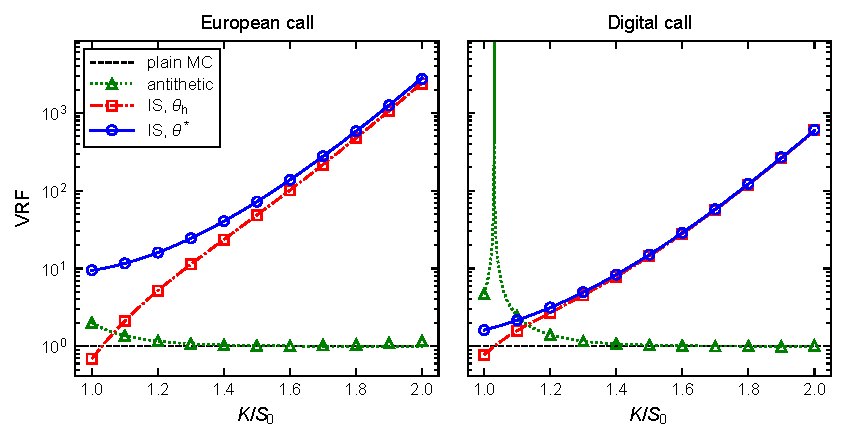
\includegraphics{e1_vrf_against_moneyness}
\caption{Variance reduction factor against the moneyness $K/S_0$, with $n = 10^6$, for the call (left) and the digital (right): measured values (markers) and closed forms (lines). The dashed line is plain Monte Carlo, $\VRF = 1$.}
\label{fig:e1}
\end{figure}

The first thing to notice in Figure~\ref{fig:e1} is the scale. With the optimal drift, the VRF goes from $9.5$ for the call and $1.6$ for the digital at $K/S_0 = 1$ to about $2700$ and $600$ at $K/S_0 = 2$ (measured, $2735$ and $607$, against $2804$ and $593$ in closed form), that is, a gain of three orders of magnitude over plain Monte Carlo for the call and of more than two for the digital, whereas antithetic variates go from $2.0$ and $4.7$ down to one. Is the size of this growth a coincidence? It is not. For the digital with the heuristic drift, \eqref{eq:M2-dig} at $a = -d_2$ and the Mills ratio give $\VRF(\theta_{\mathrm h}) \sim 2e^{d_2^2/2}$ as $d_2 \to -\infty$,\footnote{The relative variance per sample of plain Monte Carlo is $(1-p)/p \sim \sqrt{2\pi}\,|d_2|\,e^{d_2^2/2}$, and that of importance sampling is $e^{d_2^2}N(2d_2)/N(d_2)^2 - 1 \sim \frac{\sqrt{2\pi}}{2}\,|d_2|$, both because $N(x) \sim \varphi(x)/|x|$ as $x \to -\infty$. The VRF is their ratio.} and since $d_2$ is affine in $\log(K/S_0)$, on the logarithmic axis of the figure the curve bends upwards like a parabola in the log-moneyness. Put differently, the relative variance of plain Monte Carlo grows exponentially in $d_2^2$, while that of importance sampling grows only like $|d_2|$: the drift does not remove the difficulty of the rare event, but it does remove its exponential part.

The heuristic deserves a closer look, since it is the curve that tells the most. At $K/S_0 = 1$ it is below one, $0.69$ for the call and $0.77$ for the digital, so there importance sampling with $\theta_{\mathrm h}$ is worse than doing nothing. This is not a defect of the code but what Subsection~\ref{subsec:heur} predicts, since with $d_2 > 0$ the heuristic drift is negative. The curve equals one where $d_2 = 0$, that is, at $K/S_0 = e^{(r - \sigma^2/2)T}$, just above one and before the second strike of the figure, where the drift vanishes, and from there on it behaves differently for each payoff. For the digital it stays close to the optimum ($14.4$ against $15.0$ at $K/S_0 = 1.5$, and $585$ against $593$ at $K/S_0 = 2$, in closed form), as Proposition~\ref{prop:digopt} predicts, whereas for the call it falls well short of it ($48.5$ against $72.4$, and $2438$ against $2804$), for the reason given in Subsection~\ref{subsec:heur-opt}: the region that matters lies above $K$.

Antithetic variates behave just as Section~\ref{sec:mc} anticipated. At $K/S_0 = 1$ they give $2.00$ for the call, the value measured in \cite{portfolio}, and $4.69$ for the digital, and out of the money both curves fall to one, as Proposition~\ref{prop:av-otm} says they must, since a path and its antithetic partner are then never both in the money. One feature of the figure may look like an error and is not: the curve of the digital shoots up just above $K/S_0 = 1$. Where $d_2 = 0$, the events $\{Z > -d_2\}$ and $\{-Z > -d_2\}$ are complementary (up to a null set), so exactly one member of each pair ends in the money, $g(Z) + g(-Z) = e^{-rT}$ is constant, and the antithetic estimator has zero variance, which makes its VRF infinite at that strike.\footnote{The closed curve is computed from Proposition~\ref{prop:av} by quadrature, on a grid refined around that strike, which is why it leaves the frame.} As for who wins where, for the digital antithetic variates are the best method at $K/S_0 = 1.0$ and $1.1$, and importance sampling from $1.2$ on, while for the call the optimal drift wins at every strike and the heuristic from $1.1$ on. Rather than a race, then, the figure shows a division of labour: antithetic variates work near the money, precisely where the heuristic drift fails, and importance sampling works out of the money, precisely where antithetic variates give nothing.

Finally, the measured points follow the closed curves to within $0.6\%$ up to $K/S_0 = 1.5$, and to within $3\%$ for importance sampling at $K/S_0 = 2$, but at that strike the antithetic point of the call is at $1.17$ instead of $1.00$. One might be tempted to think that the antithetic estimator misbehaves there. It does not, and the reason is in the measured variances, not in the estimator. The VRF is a ratio of two measured variances, and at $K/S_0 = 2$ both rest on the few hundred samples, out of $10^6$, that end in the money, the antithetic one through the pairs they belong to, and for the call on the largest payoffs among them. The precision of a measured variance is governed by the fourth moment of the samples, with a relative error of $\sqrt{(\kappa - 1)/n}$, where $\kappa$ is the kurtosis, and $\kappa$ is very large precisely when the variance is carried by a few rare values. Which of the two is off, then? Since the estimators share the draws, the same plain variance is the numerator of the three VRFs of the call, and the two points of importance sampling, whose own variance rests on the many samples that the drift sends into the money and so is measured precisely, are within $3\%$ of their curves. The plain variance is therefore close to its true value, and it is the antithetic one that is off. Table~\ref{tab:e4}, with its own draws, gives $0.81$ for the same point.

\subsection{The role of the drift}
\label{subsec:drift}

\begin{figure}[t]
\centering
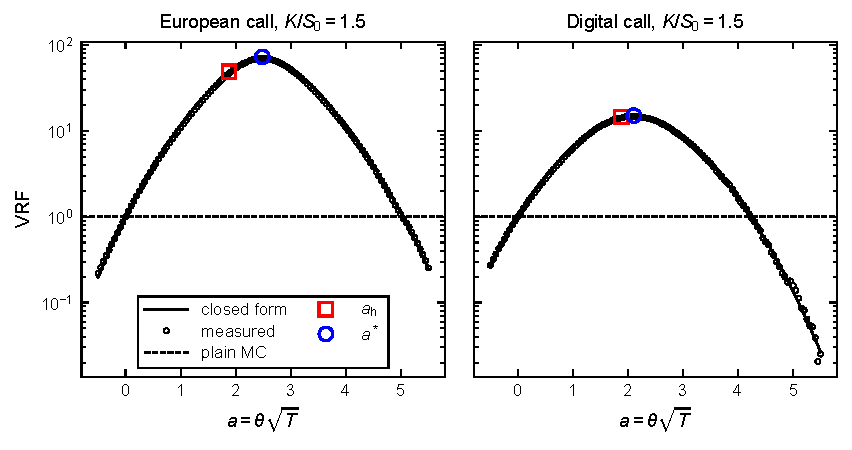
\includegraphics{e2_vrf_against_drift}
\caption{Variance reduction factor of importance sampling against the drift $a = \theta\sqrt T$ at $K/S_0 = 1.5$, with $n = 10^5$ and the same draws for every $a$: closed form (line) and measured values (circles), with $a_{\mathrm h}$ and $a^*$ marked.}
\label{fig:e2}
\end{figure}

Figure~\ref{fig:e2} is a slice of Figure~\ref{fig:e1} along the drift, at $K/S_0 = 1.5$, and \eqref{eq:chi2} says what it measures. Since the relative variance per sample is $\chi^2(q^* \,\|\, q_\theta)$, the VRF at drift $a$ is $\chi^2(q^* \,\|\, q_0)/\chi^2(q^* \,\|\, q_\theta)$, so moving along the horizontal axis is moving the sampling bell $\mathcal N(a, 1)$ towards the zero-variance density $q^*$, and eventually past it. The curve starts from one at $a = 0$, and there the measured point is exactly one, since with $\theta = 0$ importance sampling is plain Monte Carlo computed from the same draws. It reaches its maximum at the optimal drift, $72.4$ for the call at $a^* = 2.48$ and $15.0$ for the digital at $a^* = 2.10$, and the heuristic, at $a_{\mathrm h} = 1.88$ for both payoffs, sits to the left of it, close for the digital ($14.4$) and further for the call ($48.5$), which is Figure~\ref{fig:e1} again at this strike.

Why does the curve have this shape? By Theorem~\ref{thm:thetastar}, $M_2$ is strictly convex and tends to infinity on both sides, so the VRF has a single maximum, at $a^*$, and tends to zero at both ends. It is below one for every $a < 0$, because $a^* > 0$: indeed, $M_2'(0) = -\E_\Q[\Wt_T Y^2] < 0$, since $Y^2$ is nondecreasing in $\Wt_T$ and so positively correlated with it (Chebyshev's covariance inequality), and a convex function that decreases at $0$ attains its minimum to the right of it. On the right, the curve falls below one again from $a \approx 5.0$ for the call and $a \approx 4.2$ for the digital, which is the excess drift of the paragraph that follows Corollary~\ref{cor:criterion}.

The measured points follow the closed curve in the middle of the range and depart from it at the ends, by $+10.5\%$ for the call at $a = -0.5$, and for the digital by between $-35\%$ and $+20\%$ from $a = 4.9$ on, along a jagged line, although all the points use the same draws. These departures are not errors of the code but of the measured variance itself, when it rests on a few samples with large weights, and they are the subject of Section~\ref{sec:limits}.

\subsection{Cost and efficiency}
\label{subsec:cost}

We now come to the question left open in Subsection~\ref{subsec:compare}: does importance sampling not cost more? It does, and Table~\ref{tab:e4} says by how much. The times were measured on a laptop with an Intel Core i5-1135G7 processor under Windows, as the median of five runs of each estimator from the vector $Z$ to the result, so the generation of $Z$, of which antithetic variates need only half, is excluded, and so is the computation of $\theta^*$, the oracle. Plain Monte Carlo takes between $46$ and $69$ ms per $10^6$ evaluations, and relative to it importance sampling costs between $1.30$ and $1.74$ times as much, and antithetic variates between $0.98$ and $1.20$. The extra cost of importance sampling is the weight \eqref{eq:weight}, one exponential and one product per evaluation, and it does not depend on $\theta$, as we noted at the beginning of Section~\ref{sec:theta}. The two drifts should therefore cost the same, and the fact that their measured costs differ by up to $0.18$ tells us how noisy these timings are: differences of efficiency of that order, such as $346$ against $342$ for the digital at $K/S_0 = 2$, mean nothing.

With this in mind, the efficiency $\Eff = \VRF/c$ of \eqref{eq:eff} answers the question. With the optimal drift it goes from $6.4$ for the call and $1.1$ for the digital at $K/S_0 = 1$ to $1610$ and $342$ at $K/S_0 = 2$. Out of the money, then, the extra cost is irrelevant against gains in the hundreds or thousands, while near the money it can eat most of a small gain, as for the digital at $K/S_0 = 1$, whose VRF of $1.61$ becomes an efficiency of $1.12$. The heuristic at $K/S_0 = 1$ has both its variance and its cost against it, and its efficiency drops to $0.53$ for the call and $0.54$ for the digital. Antithetic variates cost about as much as plain Monte Carlo, so their efficiency stays close to their VRF ($2.03$ and $4.00$ at $K/S_0 = 1$, against VRFs of $2.00$ and $4.67$), and at $K/S_0 = 2$ their measured VRF, $0.81$ for the call and $0.92$ for the digital instead of about one, shows the same noise as Figure~\ref{fig:e1}. As for the estimates themselves, $31$ of the $32$ lie within their $95\%$ half-width of the exact price, and the exception, the digital at $K/S_0 = 1.2$ with $\theta^*$, lies at $1.04$ half-widths, that is, at $2.0$ standard errors: just what one expects of $32$ intervals at $95\%$, and far from the four standard errors of Subsection~\ref{subsec:validation}.

\subsection{Deep out of the money}
\label{subsec:deep}

\begin{figure}[t]
\centering
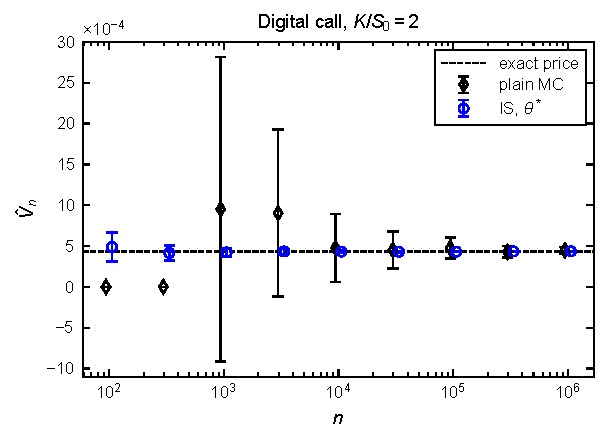
\includegraphics{e3_estimate_against_n}
\caption{Digital at $K/S_0 = 2$: estimate and $95\%$ confidence interval \eqref{eq:ci} against $n$, in units of $10^{-4}$, for plain Monte Carlo and for importance sampling with $\theta^*$. The dashed line is the exact price.}
\label{fig:e3}
\end{figure}

Figure~\ref{fig:e3} follows the digital at $K/S_0 = 2$, whose price is $V = 4.347 \times 10^{-4}$, and the first thing to notice is its left end. Plain Monte Carlo has no sample in the money at $n = 100$ and $n = 316$, an event of probability $0.955$ and $0.865$ (the CSV of the figure records both the probability and the number of hits), so its estimate is zero and its interval \eqref{eq:ci} reduces to $\{0\}$: zero width, with the price outside. With one path in the money, at $n = 1000$, the interval is $[-9.1, 28.2] \times 10^{-4}$, with a negative lower end, and so it is again with three, at $n = 3162$. Only at the right of the figure does the interval become informative, and even with $10^6$ samples, of which $469$ end in the money, its half-width is still $9\%$ of the price. This is \eqref{eq:rel-error} at work: the relative error is governed by the number of paths that end in the money, and not by $n$.

Importance sampling with the optimal drift tells a different story. Under $\Q^{\theta^*}$ more than half of the samples end in the money ($58$ out of $100$, and $56\%$ of the $10^6$), and its interval contains the price at every $n$ of the run, with a half-width of $0.38\%$ of the price at $n = 10^6$. Both half-widths fall like $n^{-1/2}$, by \eqref{eq:se}, and at equal $n$ their ratio is $\sqrt{\VRF}$, so importance sampling reaches the precision that plain Monte Carlo has at $n = 10^6$ with about $600$ times fewer samples (between $n = 10^3$ and $10^{3.5}$ in the figure), which is its VRF at this strike in Table~\ref{tab:e4}. Why the interval of plain Monte Carlo fails at the left of the figure, and what a single run can and cannot say about an interval, is the subject of Section~\ref{sec:limits}.

\section{Limitations and outlook}
\label{sec:limits}

This last section is a synthesis, and it has three parts. The first looks back at the two places where Section~\ref{sec:results} found the measurements departing from the closed forms, the left end of Figure~\ref{fig:e3} and the ends of Figure~\ref{fig:e2}, and shows that they are one and the same failure: the variance is produced in a region that the sampling law rarely visits, and a sample that has not visited it cannot estimate it. The second says what can be done about it, for the interval of the digital and for the choice of $\theta$ when there is no closed form, and the third looks beyond the European payoffs of this note.

\subsection{The interval without hits}
\label{subsec:nohits}

The left end of Figure~\ref{fig:e3} is the place to start. Let $K_n$ be the number of samples that end in the money among $n$. Under $\Q$ each of them does so independently with probability $p = N(d_2)$, so $K_n$ is binomial and $\Q(K_n = 0) = (1 - p)^n \approx e^{-np}$, which is the $0.955$ and $0.865$ of Subsection~\ref{subsec:deep} at $n = 100$ and $n = 316$. What does the interval \eqref{eq:ci} report then? Every $Y_i$ is zero, so $\hat V_n = 0$ and $s_n = 0$, and the interval reduces to $\{0\}$: it does not merely miss the price, it claims total precision. The reason is that $s_n^2$ estimates $\sigma_Y^2 = \E_\Q[Y^2] - V^2$ by plugging in the sample, and for the digital $\E_\Q[Y^2] = e^{-2rT}p$ comes entirely from the event $\{S_T > K\}$, so a sample with no hits has never visited the only region that produces variance, and it estimates the variance by zero. Nothing in \eqref{eq:ci} warns about this, since the interval is justified asymptotically and has no way of telling that the asymptotic regime has not been reached. In particular, since an interval $\{0\}$ never contains $V > 0$, the coverage is at most $\Q(K_n \ge 1) = 1 - (1 - p)^n$, that is, $4.5\%$ at $n = 100$ and $13.5\%$ at $n = 316$.

With a few hits the interval exists, but the following proposition shows what it is worth.

\begin{proposition}\label{prop:khits}
For the digital, let $K_n = k \ge 1$. Then $\hat V_n = e^{-rT}k/n$, and the interval \eqref{eq:ci} is
\begin{equation}\label{eq:khits}
  \hat V_n\,\bigl[\,1 - z\rho_{n,k},\ 1 + z\rho_{n,k}\,\bigr],
  \qquad
  \rho_{n,k} \eqdef \sqrt{\frac{n - k}{(n-1)\,k}} .
\end{equation}
\end{proposition}

\begin{proof}
Each $Y_i$ is either $e^{-rT}$ or $0$, so $\sum_i Y_i^2 = e^{-2rT}k$ and $s_n^2 = \bigl(\sum_i Y_i^2 - n\hat V_n^2\bigr)/(n-1) = e^{-2rT}k(n-k)/\bigl(n(n-1)\bigr)$. The half-width $z s_n/\sqrt n$ is then $z\rho_{n,k}\hat V_n$.
\end{proof}

Three consequences of \eqref{eq:khits} can be read in Figure~\ref{fig:e3}. With a single hit, $\rho_{n,1} = 1$ whatever $n$ is, so the interval is $[1 - z, 1 + z]\,\hat V_n$, with a negative lower end, and this is the $[-9.1, 28.2] \times 10^{-4}$ of $n = 1000$. More generally, the lower end is negative if and only if $z\rho_{n,k} > 1$, that is, $k < z^2 n/(n - 1 + z^2)$, which for every $n$ between $10^2$ and $10^6$ means at most three hits, as happens again at $n = 3162$. Finally, for $k \ll n$ we have $\rho_{n,k} \approx 1/\sqrt k$, so the relative half-width is about $z/\sqrt k$, a function of the number of hits and not of $n$, which is \eqref{eq:rel-error} read on the sample, since $np = \E[K_n]$. The coverage of the interval depends on the number of hits as well, and the next proposition makes this precise.

\begin{proposition}\label{prop:poisson}
Let $n \to \infty$ and $p = p_n \to 0$ with $np_n \to \nu \in (0, \infty)$. Then the coverage of \eqref{eq:ci} for the digital converges to
\[
  \gamma(\nu) \eqdef \Pr\bigl(J \ge 1,\ |J - \nu| \le z\sqrt{J}\bigr), \qquad J \sim \mathrm{Poisson}(\nu),
\]
for every $\nu$ such that no integer $k$ satisfies $|k - \nu| = z\sqrt k$.
\end{proposition}

\begin{proof}
By Proposition~\ref{prop:khits}, the interval contains $V$ if and only if $K_n \ge 1$ and $|K_n - np_n| \le z\sqrt{K_n(n - K_n)/(n-1)}$. For each fixed $k$, $\Pr(K_n = k) \to e^{-\nu}\nu^k/k!$ by the law of small numbers, and the condition converges to $|k - \nu| \le z\sqrt k$, which is not an equality by assumption. Since the laws of the $K_n$ are tight, summing over $k$ gives the limit.
\end{proof}

Out of the money, then, the coverage of the interval is a function of $\nu = np$ alone, the expected number of hits. For $\nu \ll 1$ it is about $1 - e^{-\nu} \approx \nu$, the probability of having any hit at all, it approaches $95\%$ only as $\nu$ grows, and even then the interval may cover the price and still be useless, with a relative half-width of $z/\sqrt k$. Put differently, what the central limit theorem needs to be large is $np$, and not $n$. The Berry--Esseen theorem says the same thing in general: for i.i.d.\ summands, the distance between the law of $\sqrt n(\hat V_n - V)/\sigma_Y$ and the standard normal law is at most $C_{\mathrm{BE}}\,\E|Y - V|^3/(\sigma_Y^3\sqrt n)$, with $C_{\mathrm{BE}}$ an absolute constant, and for the digital this bound is of the order of $1/\sqrt{np}$.

\subsection{What a single run says}
\label{subsec:single-run}

Figure~\ref{fig:e3} also shows the interval of importance sampling containing the price at every $n$, with $58$ of the $100$ samples in the money at $n = 100$. It is natural to ask, then, whether this means that the interval is reliable from $n = 100$ on. Not by itself. The $95\%$ of \eqref{eq:ci} is a property of the procedure (Section~\ref{sec:mc}), and a single run, even one in which the interval always covers, is one draw of it. What can be said is why one expects the interval to be reliable, and for that the number of hits has to be extended to weighted samples.

\begin{proposition}\label{prop:neff}
Let $X_1, \dots, X_n \ge 0$ be i.i.d.\ replications of an estimator of $V$ ($X_i = Y_i$ for plain Monte Carlo, $X_i = Y_i^\theta$ for importance sampling), with $\sum_i X_i > 0$, and let $n_{\mathrm{eff}} \eqdef \bigl(\sum_i X_i\bigr)^2/\sum_i X_i^2$. Then the relative half-width of the interval \eqref{eq:ci} built from them is
\begin{equation}\label{eq:neff}
  z\,\sqrt{\frac{n}{n-1}\Bigl(\frac{1}{n_{\mathrm{eff}}} - \frac1n\Bigr)} .
\end{equation}
For the digital under $\Q$, $n_{\mathrm{eff}} = K_n$. As $n \to \infty$, $n_{\mathrm{eff}}/n \to V^2/M_2(\theta) = 1/\bigl(1 + \chi^2(q^* \,\|\, q_\theta)\bigr)$ almost surely.
\end{proposition}

\begin{proof}
With $\bar X$ the sample mean, $s_n^2 = \frac{n}{n-1}\bigl(\frac1n\sum_i X_i^2 - \bar X^2\bigr)$, so
\[
  \frac{s_n^2}{n\bar X^2} = \frac{1}{n-1}\Bigl(\frac{n\sum_i X_i^2}{(\sum_i X_i)^2} - 1\Bigr) = \frac{n}{n-1}\Bigl(\frac{1}{n_{\mathrm{eff}}} - \frac1n\Bigr),
\]
which is \eqref{eq:neff} squared and divided by $z^2$. For the digital, $\sum_i X_i = e^{-rT}K_n$ and $\sum_i X_i^2 = e^{-2rT}K_n$. The limit is the strong law of large numbers in the numerator and the denominator, together with \eqref{eq:chi2}, which gives $M_2/V^2 = 1 + \chi^2$.
\end{proof}

We call $n_{\mathrm{eff}}$ the effective number of hits, since it extends the number of hits to any payoff and any weights: as far as its interval is concerned, every estimator of this note behaves like a plain digital with $n_{\mathrm{eff}}$ hits, and for $n_{\mathrm{eff}} \ll n$ its relative half-width is about $z/\sqrt{n_{\mathrm{eff}}}$, just as in Proposition~\ref{prop:khits}. For plain Monte Carlo on the digital $n_{\mathrm{eff}}/n \to p$, which out of the money is tiny, whereas for importance sampling $n_{\mathrm{eff}}/n \to 1/(1 + \chi^2)$, so the $\chi^2$ distance of Section~\ref{sec:theta} is precisely what decides how many effective hits a drift buys. Under the optimal drift at $K/S_0 = 2$ more than half of the samples end in the money and $n_{\mathrm{eff}}$ grows like a fixed fraction of $n$, instead of like $np$, so the failure of Subsection~\ref{subsec:nohits} disappears and one expects the interval to be close to nominal from small $n$ on. We stress that this is an expectation and not a measurement, since the repository measures coverage only at $K/S_0 = 1.2$ and $1.5$ (Subsection~\ref{subsec:validation}). Note, finally, that $n_{\mathrm{eff}}$ is computed from the sample, so it inherits the blindness of Subsection~\ref{subsec:nohits}: a sample that has missed the region that produces the variance overestimates $n_{\mathrm{eff}}$, and this is the subject of the next subsection.

\subsection{Degenerate weights}
\label{subsec:weights}

Figure~\ref{fig:e2} departs from its closed curve at both ends (Subsection~\ref{subsec:drift}). Where does the variance come from at those drifts? The measure $\Q^{(2)}_\theta$ introduced after Theorem~\ref{thm:thetastar}, which weights each path by its contribution to $M_2$, answers it. For the digital, $\xi$ is under $\Q^{(2)}_\theta$ a $\mathcal N(-a, 1)$ truncated to $\xi > -d_2$, and as $a$ grows this truncated normal piles up at its truncation point, the strike: the variance is produced by the paths that end just above $K$. In the sampling coordinate $Z = \xi - a$, which is $\mathcal N(0,1)$ under $\Qt$, the strike sits at
\[
  Z = -d_2 - a = -(a - a_{\mathrm h}),
\]
so overshooting the heuristic by $\Delta = a - a_{\mathrm h}$ puts the region that produces the variance $\Delta$ standard deviations into the left tail of the sampling law, and the weights there, $e^{ad_2 + a^2/2} = e^{a(a - 2a_{\mathrm h})/2}$, are larger than one exactly when $a > 2a_{\mathrm h}$, that is, beyond the range of Remark~\ref{rem:small-weight}. This is the failure of Subsection~\ref{subsec:nohits} again, recreated by the cure: there the variance came from the money region, which $\Q$ rarely visits, and here it comes from the paths just above the strike, which $\Qt$ rarely visits. At the left end of the figure the mechanism is that of plain Monte Carlo itself, made worse by a drift that pushes the paths away from the money, and the call suffers more than the digital because its rare payoffs are also large.

A variance carried by a few samples is measured badly. As we saw in Subsection~\ref{subsec:across-strikes}, the relative error of a sample variance is $\sqrt{(\kappa - 1)/n}$, with $\kappa$ the kurtosis, and for the digital $\kappa$ grows like $e^{(a - a_{\mathrm h})^2/2}$, Gaussian in the overshoot.\footnote{Lemma~\ref{lem:gauss} gives the moments $\E_{\Qt}[(wY)^m] = e^{-mrT}e^{m(m-1)a^2/2}N\bigl(d_2 - (m-1)a\bigr)$, and the Mills ratio gives $\kappa \approx \sqrt{2\pi}\,e^{(a - a_{\mathrm h})^2/2}(a - d_2)^2/(3a - d_2)$ for large $a$.} Nor do the common draws of Figure~\ref{fig:e2} prevent the jagged line, and the reason is the payoff. For fixed $Z_1, \dots, Z_n$, the sample variance is a continuous function of $a$ for the call, whose payoff is continuous in $S_T$, but for the digital it jumps every time a sample crosses the strike, $Z_i = -d_2 - a$, and in the overshoot the samples that cross it enter with the large weights computed above. For the call, a path that enters at the strike carries a payoff close to zero and goes unnoticed, and the factor $(S_T - K)^2$ in $\Q^{(2)}_\theta$ keeps its variance away from the strike.

What does this do to the interval? In Glasserman's words, ``because likelihood ratios are often highly skewed, the sample standard deviation will often underestimate the true standard deviation, and a very large sample size may be required for confidence intervals based on the central limit theorem to provide reasonable coverage'' \cite[\S 4.6.1, p.~260]{glasserman}. A sample that misses the heavy region underestimates the price and its standard error at the same time, so the interval lies too low and is too narrow, and its misses fall below $V$. The coverage tests of Subsection~\ref{subsec:validation} pass because both drifts they use are close to the optimum, and one expects them to fail with a drift that overshoots it by much.

Without a closed form, $M_2$ is not available for comparison, and what can be monitored is the sample itself: the effective number of hits (Proposition~\ref{prop:neff}), the share of the largest term in $\sum_i X_i$, and the mean of the weights, which should be close to one, since $\E_{\Qt}[w] = 1$. None of them is a proof. No statistic computed from a sample can see a region that the sample has not visited, and the interval $\{0\}$ of Subsection~\ref{subsec:nohits} is the extreme case, since it reports zero variance. The real remedy is therefore to choose $\theta$ so that the region that produces the variance is well sampled, which is the subject of Subsection~\ref{subsec:choose}.

\subsection{Exact intervals for the digital}
\label{subsec:exact}

For the digital under $\Q$ there is a way around the central limit theorem, since $K_n$ is binomial and an interval for $p$ can be built from the binomial law itself. The Clopper--Pearson interval with $k$ hits is $[p_L, p_U]$, where $p_L$ solves $\Pr_{p_L}(K_n \ge k) = \alpha/2$ (with $p_L = 0$ if $k = 0$) and $p_U$ solves $\Pr_{p_U}(K_n \le k) = \alpha/2$, and its coverage is at least $1 - \alpha$ for every $n$ and every $p$.\footnote{The interval misses the true $p$ only if the observed count falls in the upper tail of $\mathrm{Bin}(n, p)$ of probability at most $\alpha/2$, or in its lower tail of probability at most $\alpha/2$, and each of these events has probability at most $\alpha/2$.} With no hits it reduces to $[0, 1 - (\alpha/2)^{1/n}]$, and its one-sided version at level $95\%$ gives the rule of three: $(1 - p)^n \le 0.05$ if and only if $p \ge 1 - 0.05^{1/n} \approx -\log(0.05)/n \approx 3/n$, so having seen nothing in $n$ trials we can still say, with $95\%$ confidence, that $p < 3/n$. Unlike \eqref{eq:ci}, these intervals never collapse to a point and never have a negative lower end, and with few hits they say honestly how little the sample knows. Their limitation is that they rely on the binomial structure, which only the plain digital has, and for the call, or for weighted samples, the remedy is the one this note is about, namely to sample the region that matters.

\subsection{Choosing \texorpdfstring{$\theta$}{theta} without a closed form}
\label{subsec:choose}

The heuristic is a rule for rare events and $\theta^*$ is an oracle, so neither is the end of the story in a problem without a closed form. The heuristic fails near the money, where Figure~\ref{fig:e1} shows it worse than doing nothing, for the reason given in Subsection~\ref{subsec:heur}: with $d_2 > 0$ it pushes $S_T$ down. The general rule announced there is to centre the sampling bell at the mode of the zero-variance density $q^*$, that is, to take $a$ maximising $\log g(x) - x^2/2$ \cite[\S 4.6.2, (4.90)]{glasserman}. For the digital this gives $\max(-d_2, 0)$, which is the heuristic out of the money and no shift at all near it, instead of a harmful negative one, and for the call it gives a point above $-d_2$, since $g$ grows above the strike, that is, a drift above the heuristic, in the direction of $\theta^*$. It needs neither $M_2$ nor $V$, only $g$, which is what makes it usable without a closed form.

The optimal drift, in turn, would have to be estimated, and the natural way is a pilot run. How? By \cite[(4.24)]{tfg} with reference measure $\Q^{\theta_0}$ and $X = w_\theta Y^2 \ge 0$,
\begin{equation}\label{eq:pilot}
  M_2(\theta) = \E_{\Q^{\theta_0}}\bigl[w_{\theta_0}\, w_\theta\, Y^2\bigr] \qquad \text{for every } \theta,
\end{equation}
so a single pilot sample drawn under $\Q^{\theta_0}$ estimates the whole function $\theta \mapsto M_2(\theta)$.\footnote{Here $w_\theta$ is the random variable $e^{-\theta\Wt_T + \frac12\theta^2 T}$ of \eqref{eq:weight}, with $\Wt_T = \theta_0 T + \sqrt T Z$ for the pilot draws, and not $w_\theta(Z)$, the last expression of \eqref{eq:weight} evaluated at the normal of the pilot, which is the weight of a sample drawn under $\Qt$ and not under $\Q^{\theta_0}$.} Each term is a nonnegative multiple of $e^{\theta^2 T/2 - \theta\Wt_T}$, convex in $\theta$, so the estimated function is convex and can be minimised, and the main run then uses fresh draws, as Remark~\ref{rem:same-stats} requires. Here Subsection~\ref{subsec:nohits} returns as a trap: a pilot run under $\Q$ ($\theta_0 = 0$) out of the money may have no hits, and then it estimates $M_2 \equiv 0$ for every $\theta$. It should run under the heuristic drift, or under the mode of $q^*$, which put a large share of the samples in the money. For the digital the pilot barely matters, since the heuristic is close to $\theta^*$ (Proposition~\ref{prop:digopt}), but for the call it does, as Figure~\ref{fig:e2} shows ($48.5$ against $72.4$ at $K/S_0 = 1.5$).

Does the pilot actually find $\theta^*$, and how large does it have to be? Figure~\ref{fig:e5} answers both questions at $K/S_0 = 1.5$, the strike of Figure~\ref{fig:e2}. For each payoff we draw $500$ independent pilots under $\theta_{\mathrm h}$, which sends half of the samples into the money, with sizes $m$ from $32$ to $10^4$ in steps of half a decade, and from each of them we take the drift $\hat\theta$ that minimises its estimate of $M_2$.

\begin{figure}[t]
\centering
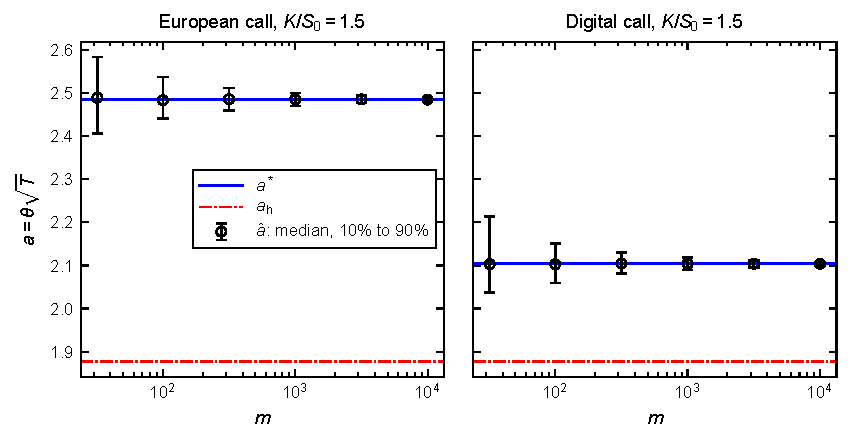
\includegraphics{e5_pilot_drift_against_m}
\caption{Pilot estimate of the optimal drift against the pilot size $m$ at $K/S_0 = 1.5$, for the call (left) and the digital (right): median and $10\%$ to $90\%$ band of $\hat a = \hat\theta\sqrt T$ over $500$ pilots under $\theta_{\mathrm h}$, with $a^*$ and $a_{\mathrm h}$ marked.}
\label{fig:e5}
\end{figure}

What is $\hat\theta$? Only the samples that end in the money contribute to the estimate, and setting to zero the derivative of its logarithm gives
\begin{equation}\label{eq:pilot-drift}
  \hat\theta\, T = \sum_i \pi_i\, \Wt_{T,i},
  \qquad
  \pi_i \propto w_{\theta_0,i}\, w_{\hat\theta,i}\, Y_i^2,
\end{equation}
where the index runs over the pilot samples in the money, and $\Wt_{T,i}$, $Y_i$ and $w_{\theta,i}$ are the values of $\Wt_T$, $Y$ and $w_\theta$ at the $i$-th of them. That is, $\hat\theta T$ is a weighted mean of their endpoints, with weights proportional to their contributions to $M_2$, which is nothing but the balance equation $\theta^* T = \E_{\Q^{(2)}_{\theta^*}}[\Wt_T]$ of Section~\ref{sec:theta} with $\Q^{(2)}_{\theta^*}$ replaced by its sample version. Two consequences follow at once: the drift exists as soon as one sample ends in the money, and it always lies above $\theta_{\mathrm h}$, since all of those samples end above the strike, which is why the band of Figure~\ref{fig:e5} never reaches $a_{\mathrm h}$.

And what does the main run gain with that drift? It uses fresh draws (Remark~\ref{rem:same-stats}), so, conditionally on the pilot, it is importance sampling with the fixed drift $\hat\theta$. By Propositions~\ref{prop:unbiased} and~\ref{prop:variance} it is then unbiased, and so unbiased unconditionally as well, with variance $\bigl(M_2(\hat\theta) - V^2\bigr)/n$, and its VRF is exactly that of Corollary~\ref{cor:criterion} at $\hat\theta$, which \eqref{eq:M2-dig} and \eqref{eq:M2-call} give in closed form. This is why the experiment needs no main run: each pilot is judged by the VRF it buys, computed exactly.

The first thing to notice in Figure~\ref{fig:e5} is that the median of $\hat a$ sits on $a^*$ from the smallest pilot on ($2.489$ against $2.485$ for the call, and $2.103$ against $2.104$ for the digital, at $m = 32$), and that the band narrows like $1/\sqrt m$, as one expects of a drift defined through sample means, from about $\pm 0.09$ at $m = 32$ to $\pm 0.005$ at $m = 10^4$. One might still ask whether the $\pm 0.05$ that a pilot of $100$ samples leaves is good enough. It is, and the reason is that $\theta^*$ is a minimum: since $M_2'(\theta^*) = 0$, an error in the drift costs a variance of second order in that error. At $m = 100$ the drifts at the two ends of the band give a VRF of $72.22$ and $72.15$ for the call, against $72.39$ at $\theta^*$ and $48.51$ at $\theta_{\mathrm h}$, and of $14.99$ for the digital, against $15.02$ and $14.44$. Put differently, a pilot of $100$ samples, one ten-thousandth of the $10^6$ samples of a main run, recovers the VRF of the oracle to within half a percent.

We stress what the figure does not show: it is limited to a single strike, and it measures neither the time of the pilot, negligible against that of the main run, nor the coverage of the interval of the main run. What it does show is that the method does not need the oracle: a short pilot under the heuristic drift finds $\theta^*$, and the closed form, still at hand in this setting, is left with a single role, that of measuring how much the pilot loses.

\subsection{Outlook}
\label{subsec:outlook}

Everything in this note rests on two simplifications, a constant drift and a payoff that depends only on $S_T$, and Remark~\ref{rem:endpoint} explains that they are what reduces the weight to a function of a single Gaussian. A barrier option breaks the second: the endpoint no longer suffices and the path has to be simulated on a time grid, and while a constant drift is still admissible by \cite[Thm~4.20]{tfg}, the best change of measure now depends on the whole path. Deterministic drifts that change over time, which Remark~\ref{rem:constant} left aside, are the natural next step, and \cite[\S 4.6.2]{glasserman} chooses them by the same rule as above, now in path space: the drift is the optimal path, the maximiser of $\log G(z) - \frac12 z^\top z$, where $G$ is the payoff as a function of the normals $z$ that drive the discretised path. More generally, the setting of this note is the first approximation of Section~\ref{sec:mc} to payoffs without a closed form \cite[\S 6.3]{tfg}. What carries over is the change of measure of Section~\ref{sec:is}, the reading \eqref{eq:chi2} of the variance as a $\chi^2$ distance, the pilot run \eqref{eq:pilot}, which Figure~\ref{fig:e5} puts to the test, and the diagnostics of Subsection~\ref{subsec:weights}, and what is lost is precisely what made Section~\ref{sec:results} possible: the closed forms that turned $\theta^*$ into an oracle and every measurement into a check against an exact value.

\clearpage
\appendix

\section{Summary table}
\label{app:table}

\begin{table}[h!]
\centering
\caption{Summary at $n = 10^6$: exact price $V$, estimate with the half-width of the $95\%$ interval \eqref{eq:ci}, variance reduction factor estimated by \eqref{eq:vrf-hat}, relative cost $c$ and efficiency $\Eff = \VRF/c$ \eqref{eq:eff}. The costs are times measured on a laptop with an Intel Core i5-1135G7 processor under Windows (median of five runs from $Z$ to the result), and they, and with them the efficiencies, change slightly from run to run, while the rest of the table is reproducible.}
\label{tab:e4}
\medskip
% Table E4, written by experiments/make_figures.py (see e4_summary.csv).
% The relative costs c, and with them the efficiencies, are times measured
% on the machine that ran the script.
\begin{tabular}{rllrrrr}
\toprule
$K/S_0$ & $V$ & estimator & estimate $\pm$ 95\% half-width & VRF & $c$ & Eff \\
\midrule
\multicolumn{7}{l}{\emph{European call}} \\
1.0 & $10.4506$ & plain MC & $10.459 \pm 0.029$ & 1.00 & 1.00 & 1.00 \\
 &  & antithetic & $10.453 \pm 0.020$ & 2.00 & 0.98 & 2.03 \\
 &  & IS, $\theta_{\mathrm{h}}$ & $10.457 \pm 0.035$ & 0.691 & 1.30 & 0.532 \\
 &  & IS, $\theta^*$ & $10.4537 \pm 0.0094$ & 9.48 & 1.48 & 6.42 \\
\addlinespace
1.2 & $3.2475$ & plain MC & $3.246 \pm 0.017$ & 1.00 & 1.00 & 1.00 \\
 &  & antithetic & $3.250 \pm 0.016$ & 1.16 & 1.02 & 1.13 \\
 &  & IS, $\theta_{\mathrm{h}}$ & $3.2516 \pm 0.0075$ & 5.19 & 1.44 & 3.60 \\
 &  & IS, $\theta^*$ & $3.2490 \pm 0.0042$ & 16.0 & 1.46 & 11.0 \\
\addlinespace
1.5 & $0.35963$ & plain MC & $0.3601 \pm 0.0056$ & 1.00 & 1.00 & 1.00 \\
 &  & antithetic & $0.3628 \pm 0.0056$ & 0.995 & 0.99 & 1.01 \\
 &  & IS, $\theta_{\mathrm{h}}$ & $0.36028 \pm 0.00080$ & 48.4 & 1.44 & 33.6 \\
 &  & IS, $\theta^*$ & $0.36007 \pm 0.00065$ & 72.4 & 1.53 & 47.2 \\
\addlinespace
2.0 & $4.799 \times 10^{-3}$ & plain MC & $(4.68 \pm 0.59) \times 10^{-3}$ & 1.00 & 1.00 & 1.00 \\
 &  & antithetic & $(5.31 \pm 0.65) \times 10^{-3}$ & 0.808 & 1.05 & 0.767 \\
 &  & IS, $\theta_{\mathrm{h}}$ & $(4.807 \pm 0.013) \times 10^{-3}$ & 2190 & 1.62 & 1360 \\
 &  & IS, $\theta^*$ & $(4.808 \pm 0.012) \times 10^{-3}$ & 2520 & 1.56 & 1610 \\
\midrule
\multicolumn{7}{l}{\emph{Digital call}} \\
1.0 & $0.53232$ & plain MC & $0.53317 \pm 0.00093$ & 1.00 & 1.00 & 1.00 \\
 &  & antithetic & $0.53257 \pm 0.00043$ & 4.67 & 1.17 & 4.00 \\
 &  & IS, $\theta_{\mathrm{h}}$ & $0.5330 \pm 0.0011$ & 0.773 & 1.42 & 0.544 \\
 &  & IS, $\theta^*$ & $0.53248 \pm 0.00073$ & 1.61 & 1.44 & 1.12 \\
\addlinespace
1.2 & $0.21226$ & plain MC & $0.21247 \pm 0.00078$ & 1.00 & 1.00 & 1.00 \\
 &  & antithetic & $0.21258 \pm 0.00066$ & 1.40 & 1.19 & 1.18 \\
 &  & IS, $\theta_{\mathrm{h}}$ & $0.21261 \pm 0.00047$ & 2.70 & 1.60 & 1.68 \\
 &  & IS, $\theta^*$ & $0.21272 \pm 0.00044$ & 3.14 & 1.58 & 1.99 \\
\addlinespace
1.5 & $0.028762$ & plain MC & $0.02881 \pm 0.00032$ & 1.00 & 1.00 & 1.00 \\
 &  & antithetic & $0.02869 \pm 0.00031$ & 1.04 & 1.04 & 1.00 \\
 &  & IS, $\theta_{\mathrm{h}}$ & $0.028809 \pm 0.000084$ & 14.5 & 1.57 & 9.20 \\
 &  & IS, $\theta^*$ & $0.028843 \pm 0.000082$ & 15.0 & 1.40 & 10.7 \\
\addlinespace
2.0 & $4.347 \times 10^{-4}$ & plain MC & $(4.36 \pm 0.40) \times 10^{-4}$ & 1.00 & 1.00 & 1.00 \\
 &  & antithetic & $(4.76 \pm 0.42) \times 10^{-4}$ & 0.916 & 1.20 & 0.762 \\
 &  & IS, $\theta_{\mathrm{h}}$ & $(4.354 \pm 0.016) \times 10^{-4}$ & 586 & 1.69 & 346 \\
 &  & IS, $\theta^*$ & $(4.355 \pm 0.016) \times 10^{-4}$ & 593 & 1.74 & 342 \\
\bottomrule
\end{tabular}

\end{table}

\begin{thebibliography}{9}

\bibitem{tfg}
R.~Cepeda Rocandio,
\emph{From the Risk-Neutral Measure to Girsanov's Theorem in Stochastic
Integration: Pricing of Financial Products},
Bachelor's thesis, University of Oviedo, 2026, cited in its version of
11 November 2026 (commit
\href{https://github.com/indexxxxbraker/option-pricing-via-martingales/tree/c0ba7d6871aaa43e29615066d5f6c0c1419f90fd}{\texttt{c0ba7d6}}).
\url{https://github.com/indexxxxbraker/option-pricing-via-martingales}

\bibitem{portfolio}
R.~Cepeda Rocandio,
\emph{Variance Reduction in Monte Carlo: Theoretical Foundations},
note in \emph{quant-finance-portfolio},
\texttt{theory/phase2/variance\_reduction\_foundations.tex}, 2026,
cited in its version of 4 November 2026 (commit
\href{https://github.com/indexxxxbraker/quant-finance-portfolio/tree/49bde78712b43860a527a96569f397a319fb673f}{\texttt{49bde78}}).
\url{https://github.com/indexxxxbraker/quant-finance-portfolio}

\bibitem{glasserman}
P.~Glasserman,
\emph{Monte Carlo Methods in Financial Engineering},
Springer, 2004.

\bibitem{asmussen-glynn}
S.~Asmussen and P.~W.~Glynn,
\emph{Stochastic Simulation: Algorithms and Analysis},
Springer, 2007.

\end{thebibliography}

\end{document}
